\documentclass[a4paper]{article}
\usepackage[title={CSE 480 Notes}]{mycommands}
\setcounter{tocdepth}{2}

\begin{document}
\tableofcontents

\section{File Types}
\subsection{CSV Files}
\begin{itemize}
    \item CSV stands for comma separated values
    \item It is a flat file format (no nesting) consisting of \emph{records} separated by newlines, with each \emph{field} separated by commas
    \begin{arrows}
        \item Fields can be enclosed in double quotes, but need not be unless a comma, double quote, or newline occurs
        \item Double quotes are escaped with another double quote
        \item Nested structure must be represented using text or strings, requiring additional parsing
    \end{arrows}
    \item The first line of the file may be a header line, providing names for each field
\end{itemize}

\subsection{JSON Files}
\begin{itemize}
    \item JSON stands for JavaScript Object Notation
    \begin{arrows}
        \item While originally derived from JavaScript, it is now a language-independent data format
    \end{arrows}
    \item Data is contained in a semi-structured hierarchical structure under one root JSON object
    \item The types in JSON are:
    \begin{itemize}
        \item \iljson{string}, a sequence of zero or more characters \iljson{"my_string"}
        \begin{arrows}
            \item Characters are escaped with \iljson{\}, such as \iljson{"}, \iljson{\}, and optionally \iljson{/}
            \item Escape sequences include backspace \iljson{\b}, formfeed \iljson{\f}, newline \iljson{\n}, carriage return \iljson{\r}, tab \iljson{\t}, and unicode \iljson{\u\#\#\#\#} where \iljson{\#\#\#\#} is a four digit hexadecimal number
        \end{arrows}
        \item \iljson{number}, a signed decimal number optionally with exponential e/E notation
        \begin{arrows}
            \item Leading zeros not allowed, except one is required before a decimal if integer part is 0
            \item Leading plus not allowed except in the exponential part
        \end{arrows}
        \item \iljson{object}, an unordered collection of name/value pairs \iljson{\{"field1": value1, "field2": value2\}}
        \item \iljson{array}, an ordered list of zero or more values of any types \iljson{[value1, value2]}
        \item \iljson{true}, \iljson{false}
        \item \iljson{null}
    \end{itemize}
    \item JSON Schema uses the following format:
    \begin{json}
{
    "title": "my_title",
    "description": "my_description",
    "type": "object"
    "properties": {
        "field1": {
            "description": "description1",
            "type": "type1"
        },
        "field2": {
            "description": "description2",
            "type": "type2"
        }
    },
    "required": ["field1", "field2"]
}
\end{json}
\item The types in JSON Schema are:
\begin{itemize}
    \item \iljson{"string"}, which keywords including \iljson{"minLength"}, \iljson{"maxLength"}, \iljson{"pattern"} (for regex), and \iljson{"format"} (for specifying specific types of strings, such as \iljson{"datetime"})
    \item \iljson{"number"} and \iljson{"integer"}, with keywords including \iljson{"minimum"}, \iljson{"maximum"}, \iljson{"exclusiveMinimum"}, and \iljson{"exclusiveMaximum"}
    \item \iljson{"object"}, where information about its contents are given by a nested schema under keyword \iljson{"properties"}
    \item \iljson{"array"}, where the schema each item must match it provided with \iljson{"items"}, and if each value must satisfy a different schema, the list of schemas is given under \iljson{"prefixItems"}
    \item \iljson{"boolean"}
    \item \iljson{"null"}, which means the data must be null
\end{itemize}
\end{itemize}

\subsection{XML File}
\begin{itemize}
    \item XML stands for eXtensible Markup Language
    \begin{arrows}
        \item HTML is a subset of XML
        \item XML is often used in web services, inter-database communication, text document formatting, and configuration files
    \end{arrows}
    \item XML also stores data in a semi-structured hierarchical structure under a single root element
    \item Each element consists of a start tag \ilxml{<tag\_name>}, optional content (without quotes), and an end tag \ilxml{</tag\_name>}, or an empty tag \ilxml{<tag\_name/>} can be used
    \item Each start or empty tag can also contain columns \ilxml{<tag\_name attr\_name="value">}
    \begin{arrows}
        \item Only one value may be specified, so if multiple are needed, oftentimes space-delimited strings are used
    \end{arrows}
    \item An XML schema uses the following format:
    \begin{xml}
<xsd:schema xmlns:xsd="schema_link">
<xsd:annotation>
  <xsd:documentation xml:lang="en">
    Description Here
  </xsd:documentation>
</xsd:annotation>
<xsd:element name="name1" type="myType1"/>
<xsd:complexType name="myType1">
  <xsd:sequence>
    <xsd:element name="name2" type="xsd:type1"/>
    <xsd:element name="name3" type="xsd:type2"/>
  </xsd:sequence>
</xsd:complexType>
</xsd:schema>
\end{xml}
    \item The built-in simple types are \ilxml{"xsd:string"}, \ilxml{"xsd:decimal"}, \ilxml{"xsd:integer"}, \ilxml{"xsd:boolean"}, \ilxml{"xsd:date"},
    \ilxml{"xsd:time"}, \ilxml{"xsd:dateTime"}, and \ilxml{"xsd:duration"}
    \item Other attributes include \ilxml{default}, \ilxml{use} (set equal to \ilxml{"required"} to make required)
    \item More detailed restrictions can be placed by defining a simple type, such as:
\begin{xml}
<xsd:simpleType name="myType">
  <xsd:restriction base="xsd:integer">
    <xsd:minInclusive value="0"/>
    <xsd:maxInclusive value="120"/>
  </xsd:restriction>
</xsd:simpleType>
\end{xml}
\end{itemize}

\section{Database Concepts}
\subsection{Introduction}
\begin{itemize}
    \item A \emph{database instance} is the actual data in a database in a moment of time, whereas a \emph{database schema} is a specification for the type of data that may be in the database
    \item \emph{Well-formed} means the data conforms to the file format, whereas \emph{valid} means the data conforms to the schema (and is well-formed)
\end{itemize}

\subsection{CAP Theorem for Distributed Databases}
\begin{itemize}
    \item A \emph{distributed database} stores information on many nodes or virtual machines
    \item The \emph{CAP Theorem} (or \emph{Brewer's Theorem}) states that a distributed database can only achieve two of the following three guarantees:
    \begin{itemize}
        \item[C:] \emph{Consistency}. The same information is seen by all clients regardless of the node accessed; all successful writes should be reflected across all nodes
        \begin{arrows}
            \item This is a different consistency then in the ACID properties
            \item A write can only be deemed successful after the information has been successfully propagated
        \end{arrows}
        \item[A:] \emph{Availability}. The database should be kept available and responsive as often as possible; any working nodes must return a valid response for any request
        \item[P:] \emph{Partition Tolerance}. The cluster should continue to work in spite of any partitions; if one part of the database is unavailable, the other parts should remain unaffected
        \begin{arrows}
            \item A \emph{partition} is a communications break within a distributed database; either a lost or delayed connection between two nodes
        \end{arrows}
    \end{itemize}
    \item This theorem yields the following cases:
    \begin{itemize}
        \item[CA:]
        \item[CP:]
        \item[AP:]
    \end{itemize}
\end{itemize}

\section{Entity-Relationship Model}
\subsection{Introduction}
\begin{itemize}
\item The \emph{entity-relationship model} is a method for describing a system as a database, and is represented using a \emph{entity-relationship diagram}
\begin{arrows}
\item An \emph{entity} is a single distinguishable thing or object, such as a student or a course offering
\item An \emph{entity set} is a collection of entities of the same type, such as all students at a university or all course offerings
\item An \emph{attribute} is a property of the entities in an entity set, such as student ID or department name (all attributes should be simple, not collections of values)
\end{arrows}
\item In an entity-relationship diagram, rectangles represent entity sets, ovals represent attributes, and diamonds represent relationships between entity sets, such as:
\begin{figure}[H]
\centering
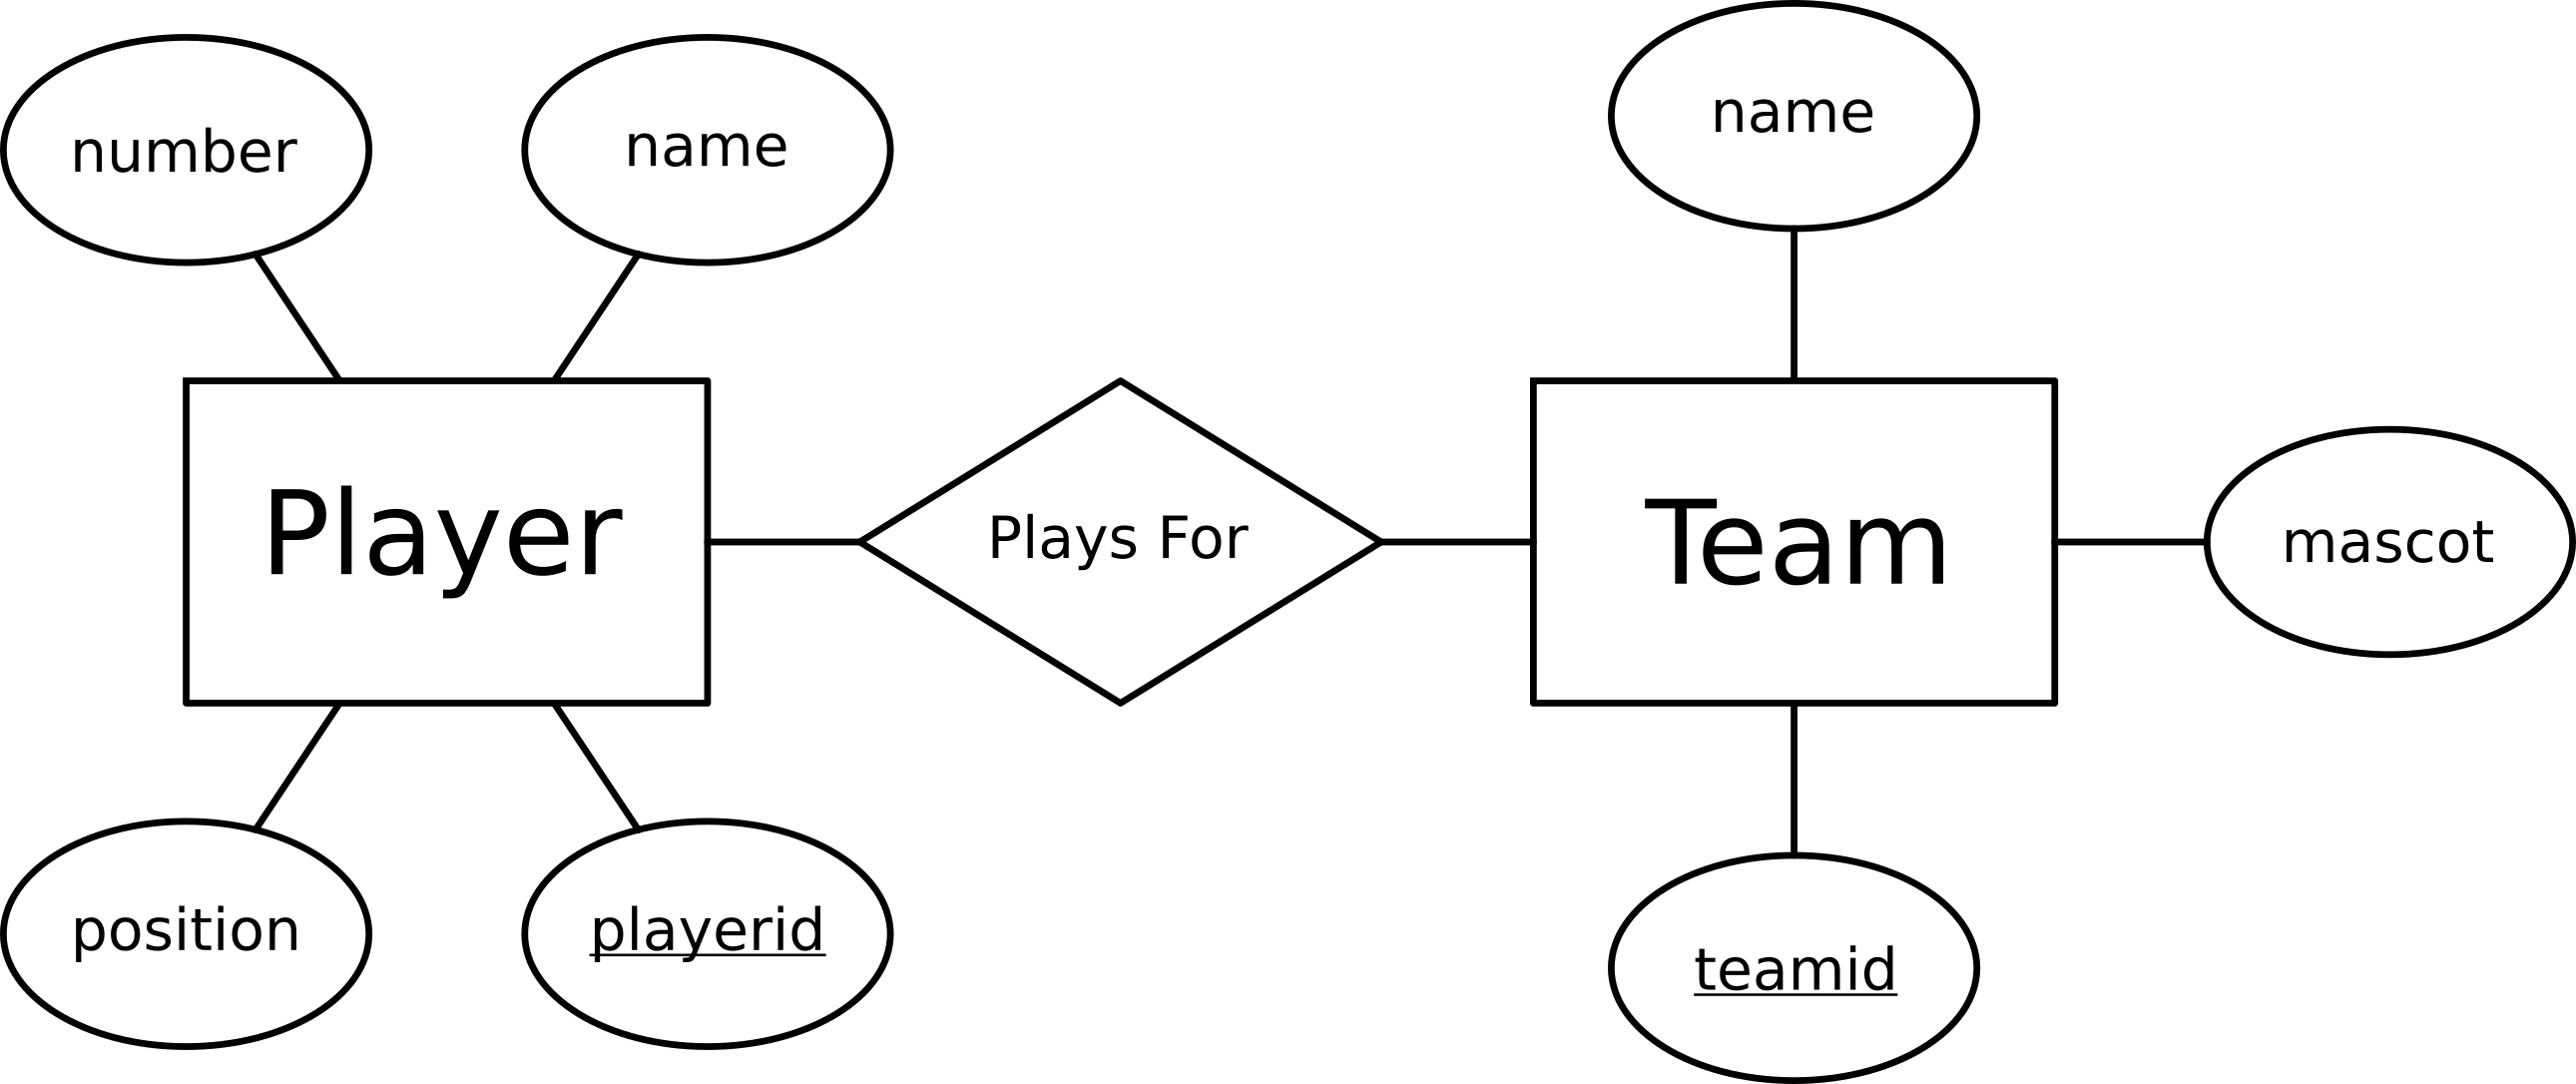
\includegraphics[width=0.5\linewidth]{entity1.png}
\end{figure}
\item Relationships can involve more than two entity sets, such as the ternary relationship:
\begin{figure}[H]
\centering
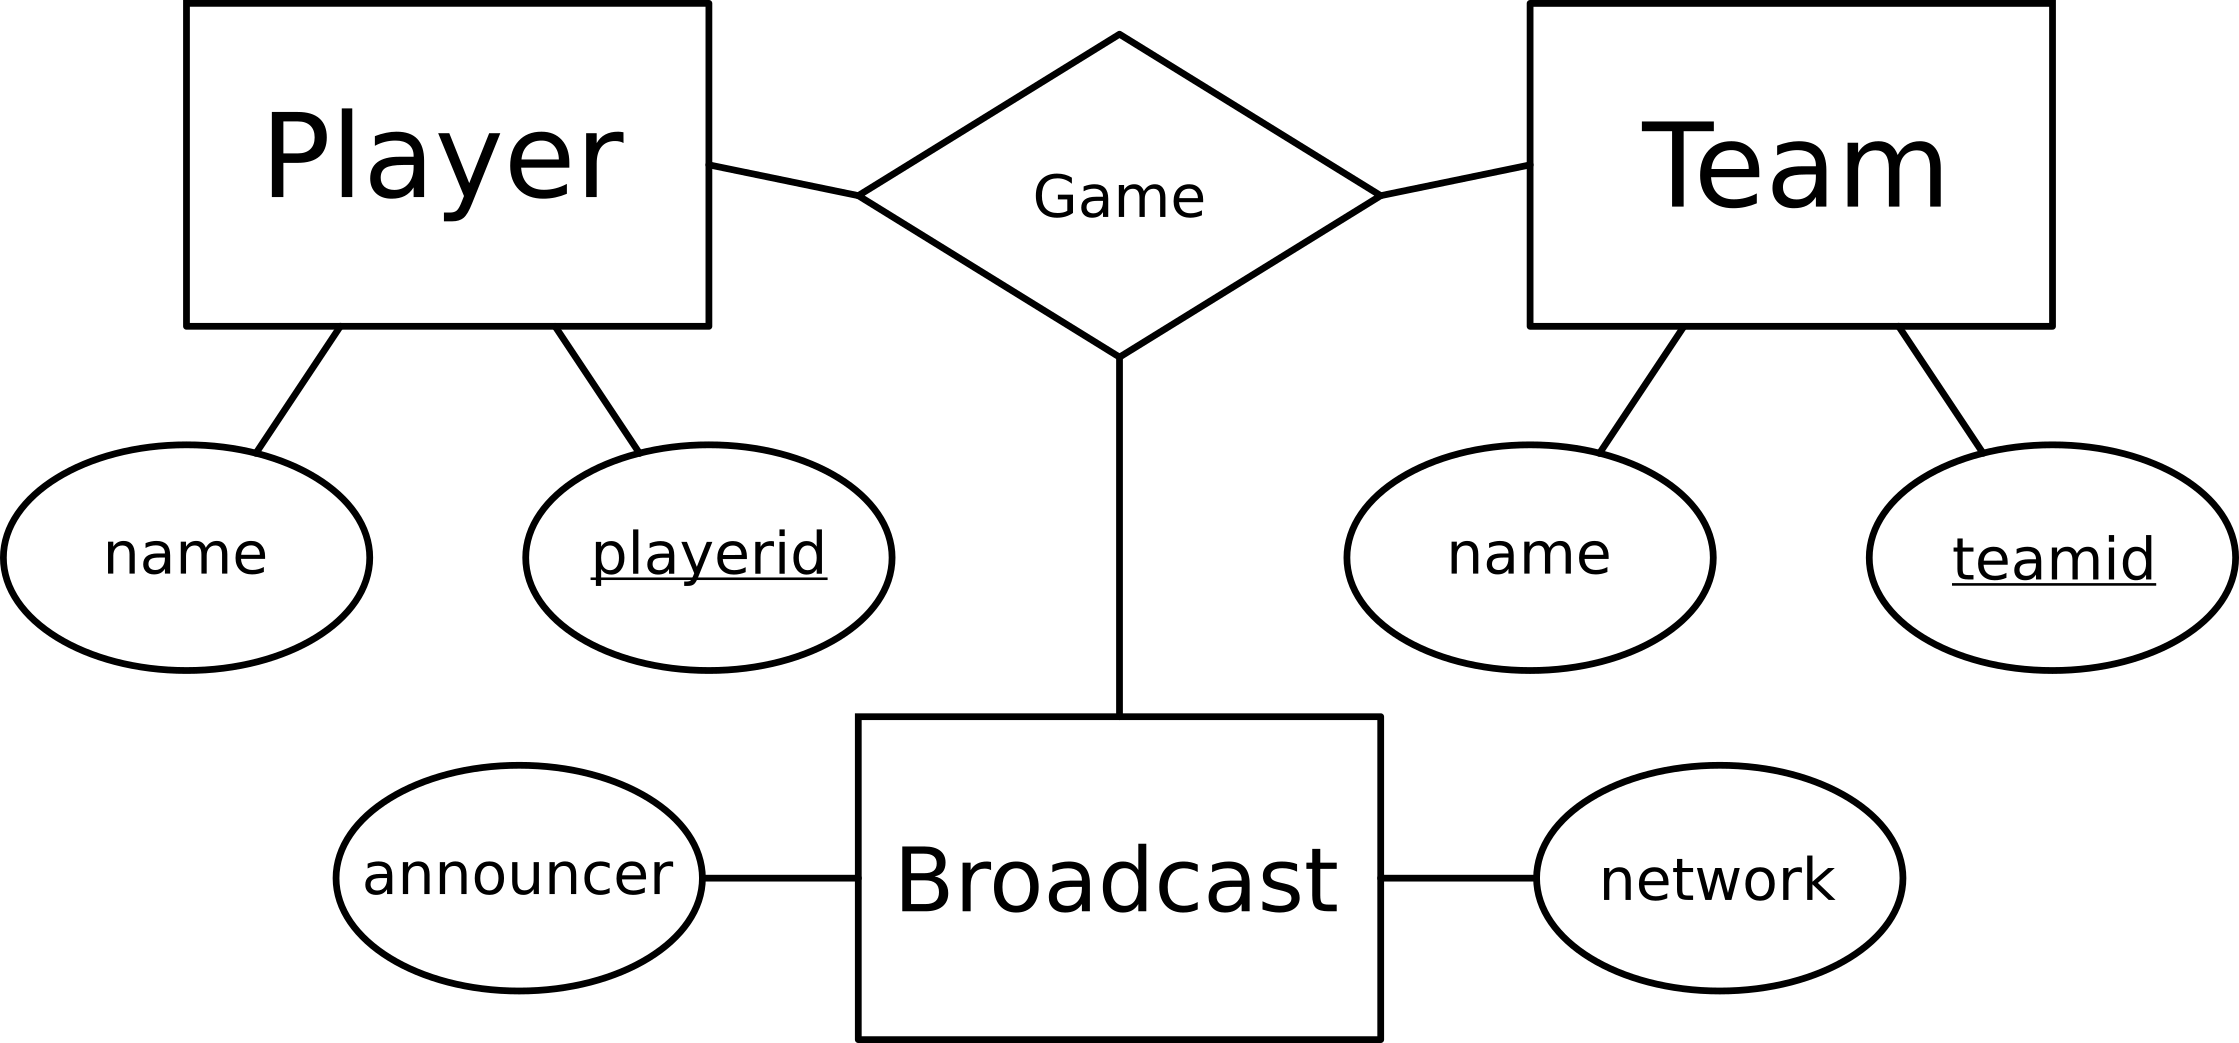
\includegraphics[width=0.5\linewidth]{entity2.png}
\end{figure}
\item The \emph{value of an entity set} is the set of entities belonging to it, and the \emph{value of a relationship set} is a set of tuples with one component for each related entity set
\begin{figure}[H]
\begin{subfigure}{0.4\linewidth}
\centering\scalebox{0.8}{
\begin{tabular}{llll}\toprule
playerid&name&number&position\\\midrule
0&Jim&5&Forward\\
1&Jane&17&Shortstop\\
2&Mary&19&Goalkeeper\\\bottomrule
\end{tabular}}
\caption*{\footnotesize Value of Team Entity Set}
\end{subfigure}%
\begin{subfigure}{0.3\linewidth}
\centering\scalebox{0.8}{
\begin{tabular}{lll}\toprule
teamid&name&mascot\\\midrule
4&Detroit&Pistons\\
9&Los Angeles&Angels\\
15&Seattle&Sounders\\\bottomrule
\end{tabular}}
\caption*{\footnotesize Value of Teams Entity Set}
\end{subfigure}%
\begin{subfigure}{0.3\linewidth}
\centering\scalebox{0.8}{
\begin{tabular}{ll}\toprule
playerid&teamid\\\midrule
0&4\\1&9\\2&15\\\bottomrule
\end{tabular}}
\caption*{\footnotesize Value of Plays For Relationship Set}
\end{subfigure}
\end{figure}
\item For a binary relationship between $A$ and $B$, the following \emph{mapping cardinalities} or \emph{multiplicities} are possible:
\begin{arrows}
\item \emph{One-to-one}, where each entity of $A$ is associated with at most one entity of $B$ and vice versa
\item \emph{One-to-many}, where each entity of $B$ is associated to at most one entity of $A$ (but any entity of $A$ can be associated to any number of entities of $B$)
\item \emph{Many-to-one}, where each entity of $A$ is associated to at most one entity of $B$ (but any entity of $B$ can be associated to any number of entities of $B$)
\item \emph{Many-to-many}, where each entity of $A$ is associated to any number of entities in $B$ and vice versa
\end{arrows}
\item If one entity is related to exactly one of another entity, this is represent with a rounded arrow
\end{itemize}

\begin{figure}[H]
\centering
\subcaptionbox*{One-to-One}[0.15\linewidth]{\centering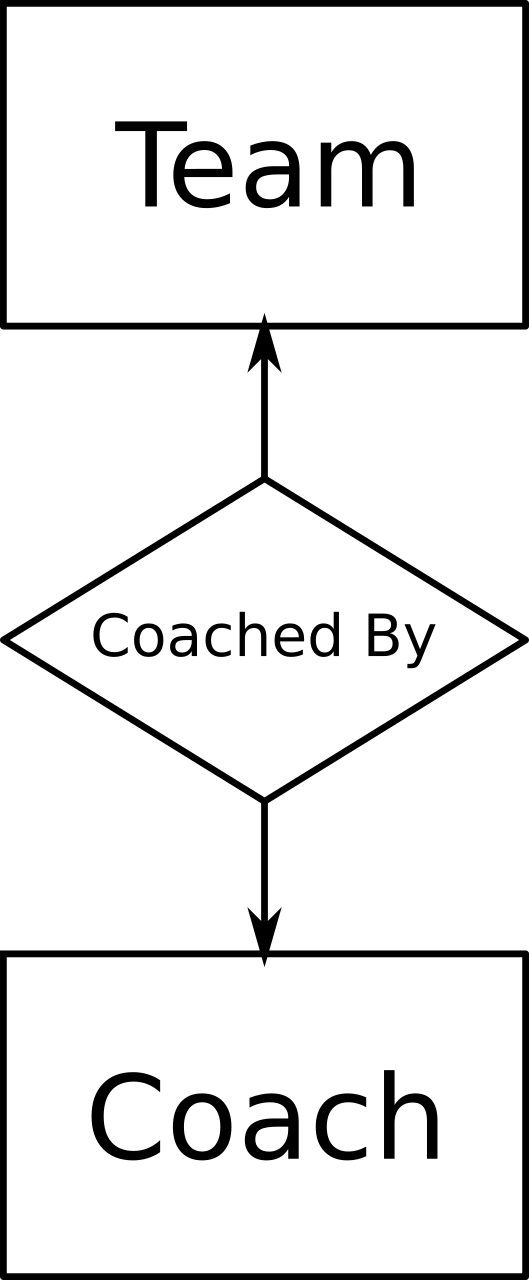
\includegraphics[width=0.6\linewidth]{entity3.png}}
\subcaptionbox*{Many-to-One}[0.15\linewidth]{\centering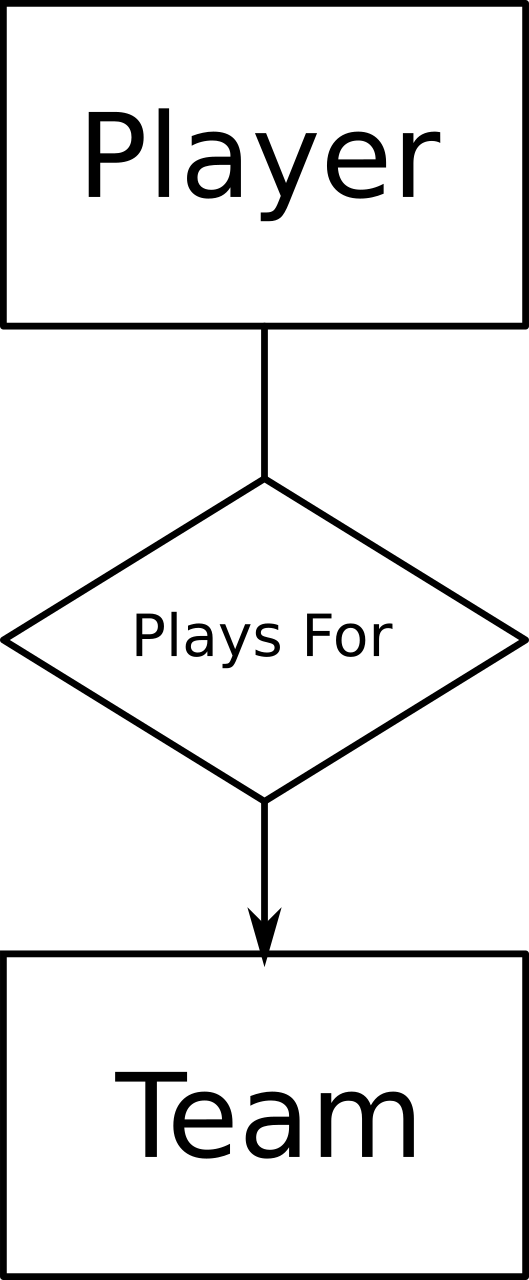
\includegraphics[width=0.6\linewidth]{entity4.png}}
\subcaptionbox*{One-to-Many}[0.15\linewidth]{\centering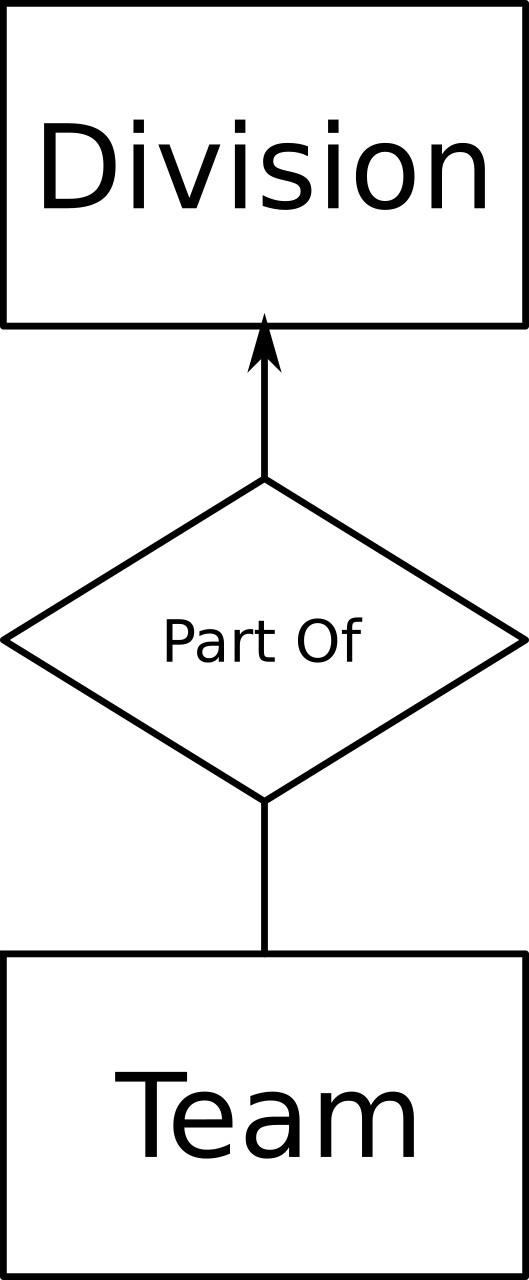
\includegraphics[width=0.6\linewidth]{entity5.png}}
\subcaptionbox*{Many-to-Many}[0.15\linewidth]{\centering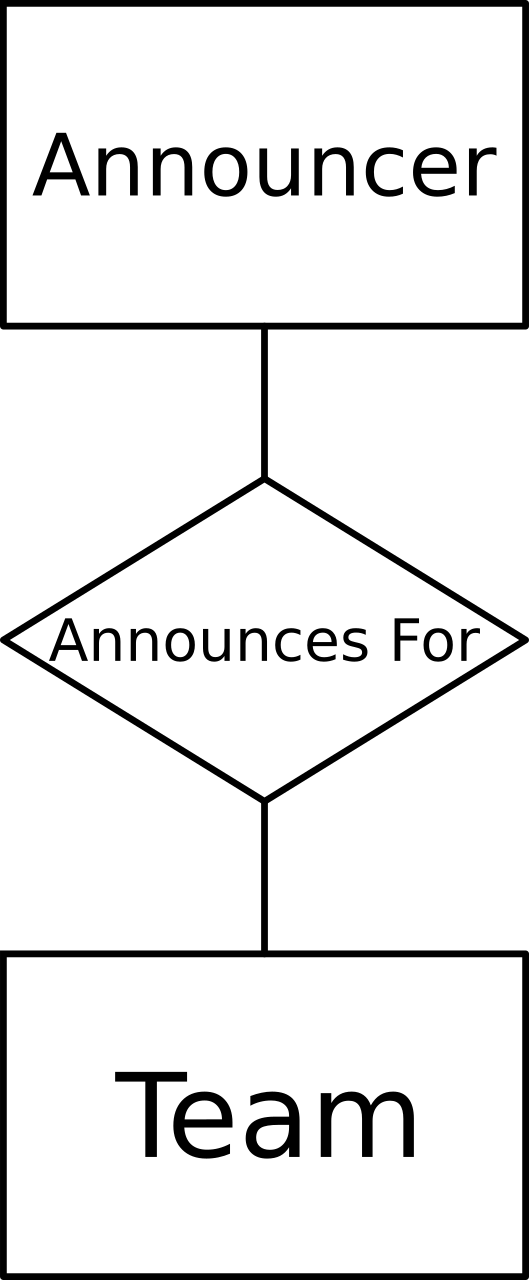
\includegraphics[width=0.6\linewidth]{entity6.png}}
\subcaptionbox*{Many-to-Exactly-One}[0.15\linewidth]{\centering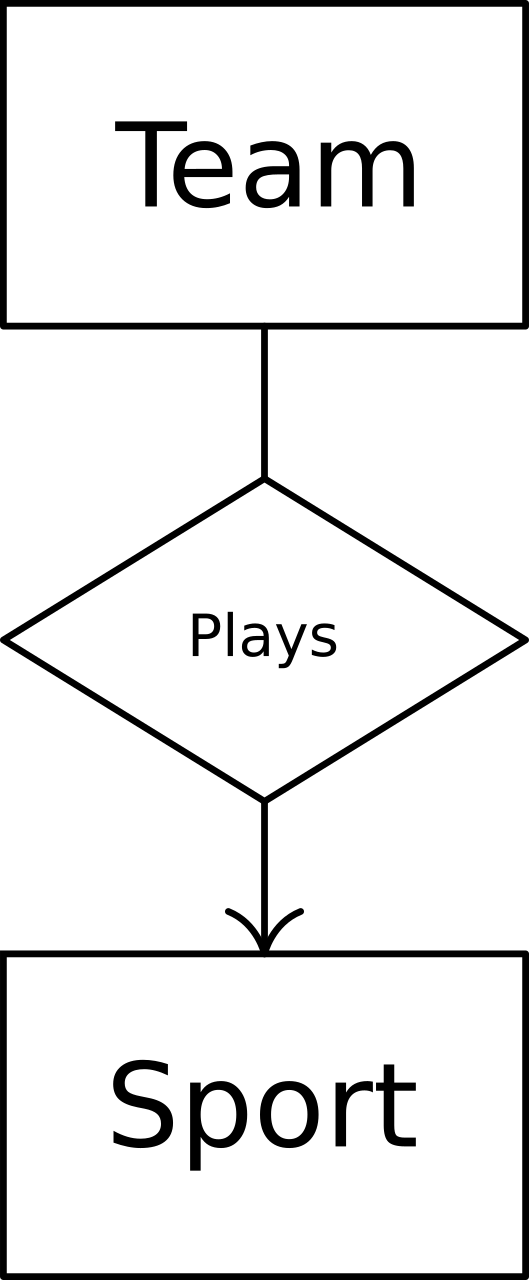
\includegraphics[width=0.6\linewidth]{entity7.png}}
\subcaptionbox*{Exactly-One-to-Exactly-One}[0.15\linewidth]{\centering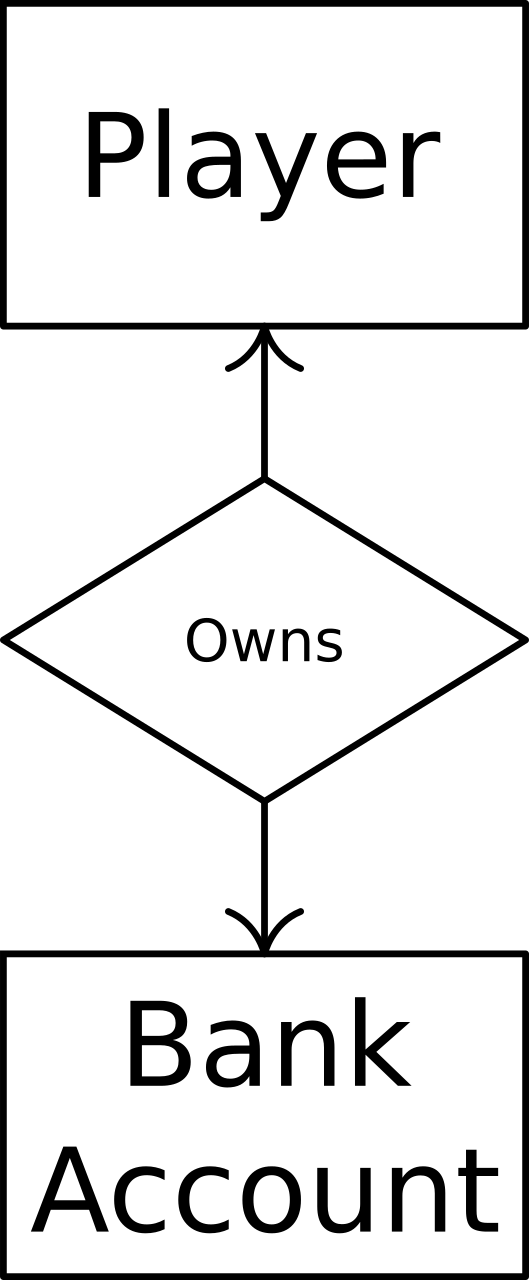
\includegraphics[width=0.6\linewidth]{entity8.png}}
\end{figure}

\begin{itemize}
\item Attributes can be present on a relationship:
\begin{figure}[H]
\centering
\begin{subfigure}{0.49\linewidth}
\centering
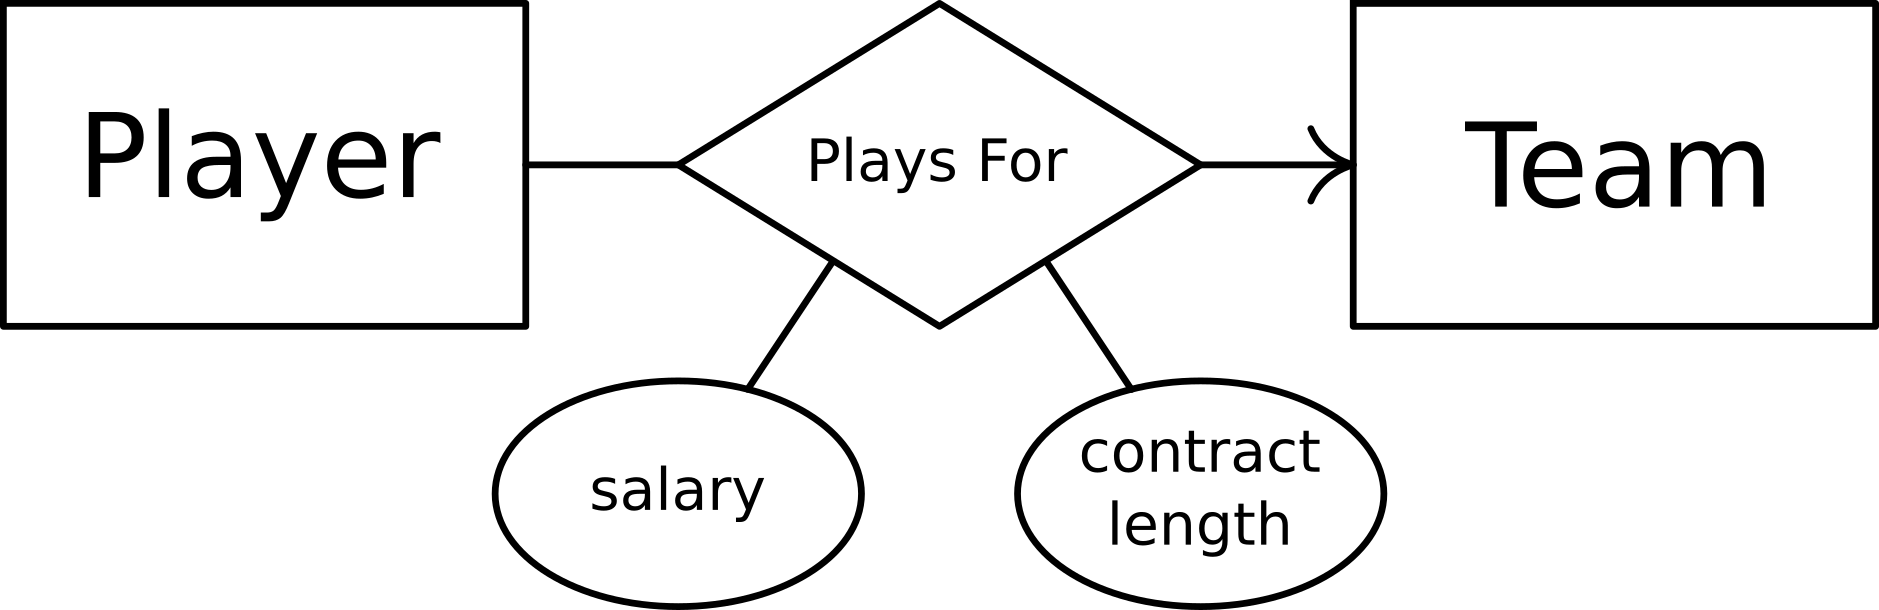
\includegraphics[width=0.9\linewidth]{entity9.png}
\caption*{Diagram with Attributes on Relationship}
\end{subfigure}
\begin{subfigure}{0.49\linewidth}
\centering
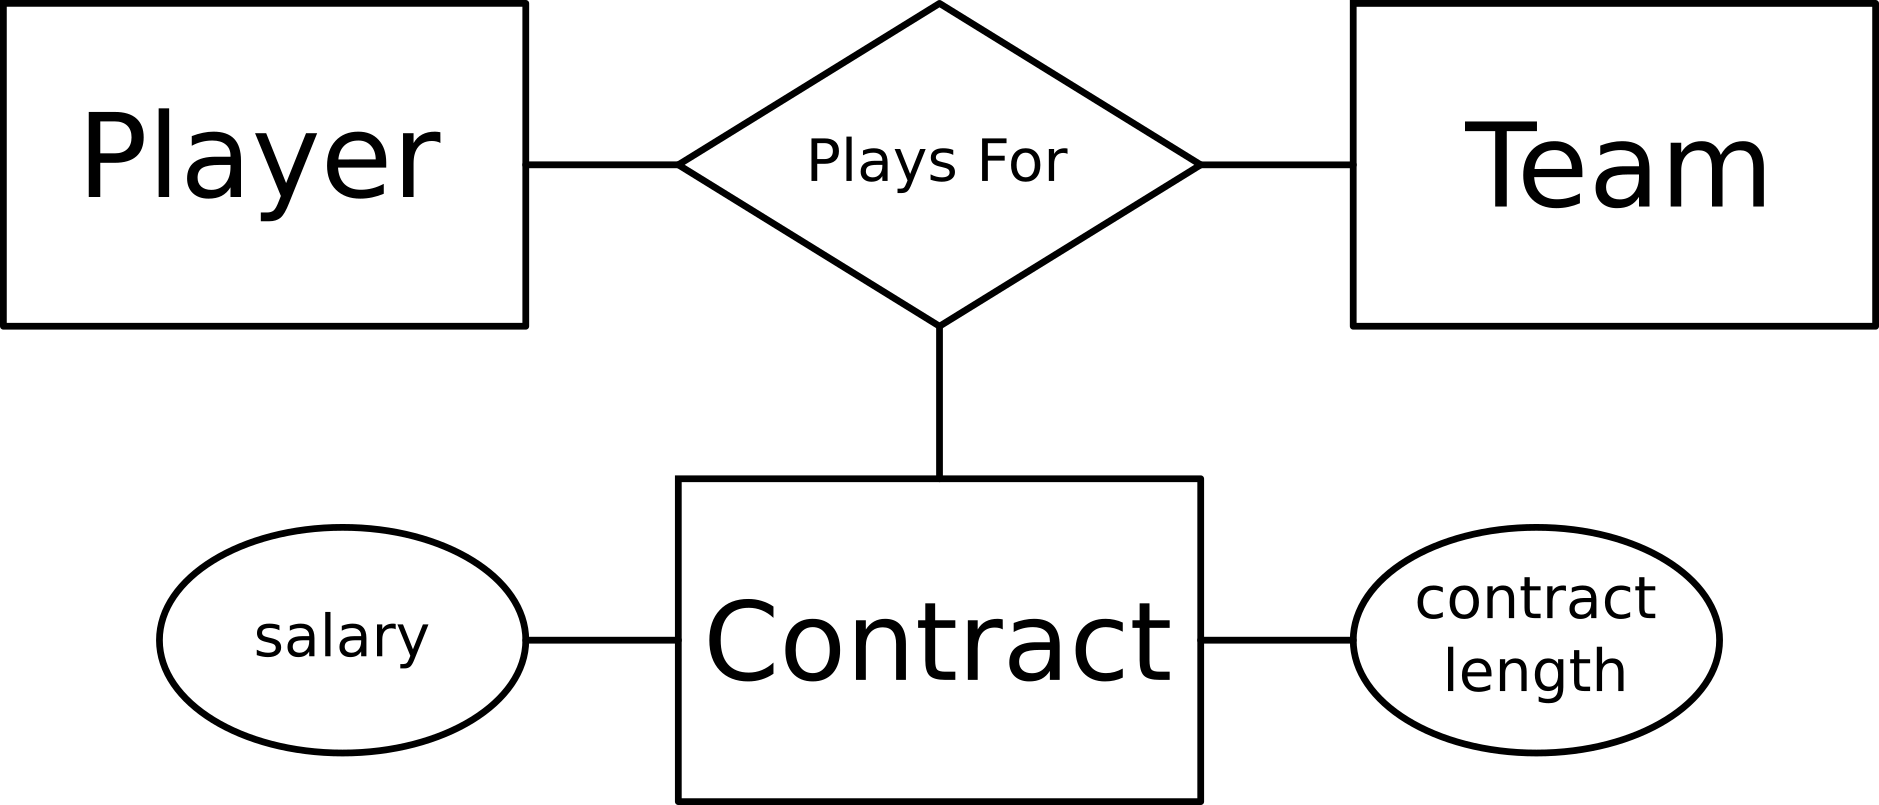
\includegraphics[width=0.9\linewidth]{entity10.png}
\caption*{Diagram without Attributes on Relationship}
\end{subfigure}
\end{figure}
\item Edges are sometimes labeled with \emph{roles} to disambiguate the case where an entity set appears multiple times in a relationship
\begin{figure}[H]
\centering
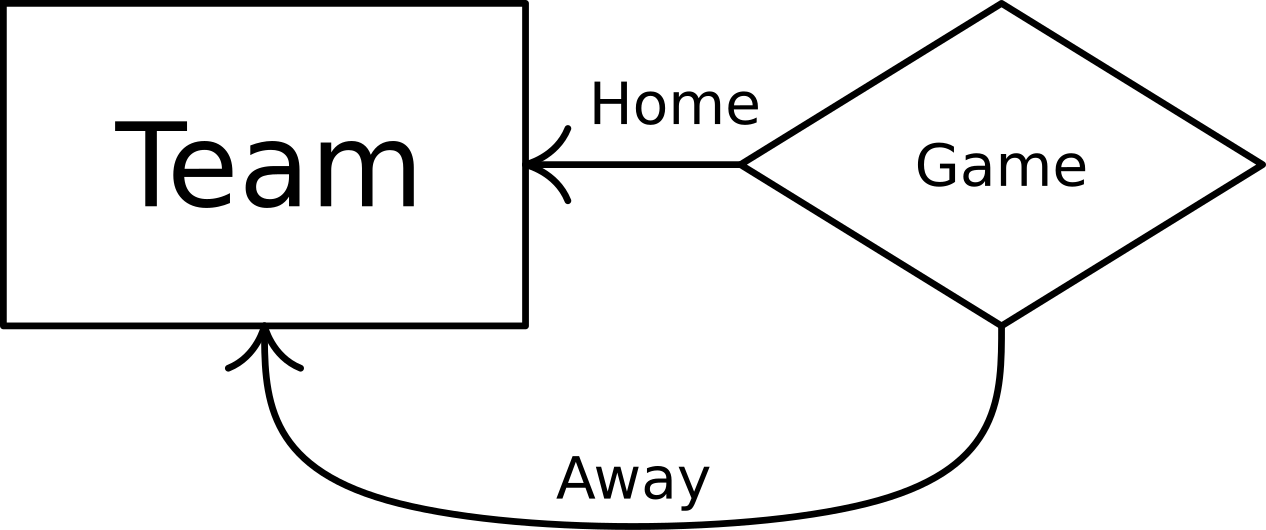
\includegraphics[width=0.3\linewidth]{entity11.png}
\end{figure}
\end{itemize}

\subsection{Subclasses}
\begin{itemize}
\item A \emph{subclass} is a special case of an entity set with more \emph{properties} (either attributes or relationships)
\begin{arrows}
\item Note that no multiple inheritance is allowed
\end{arrows}
\begin{figure}[H]
\centering
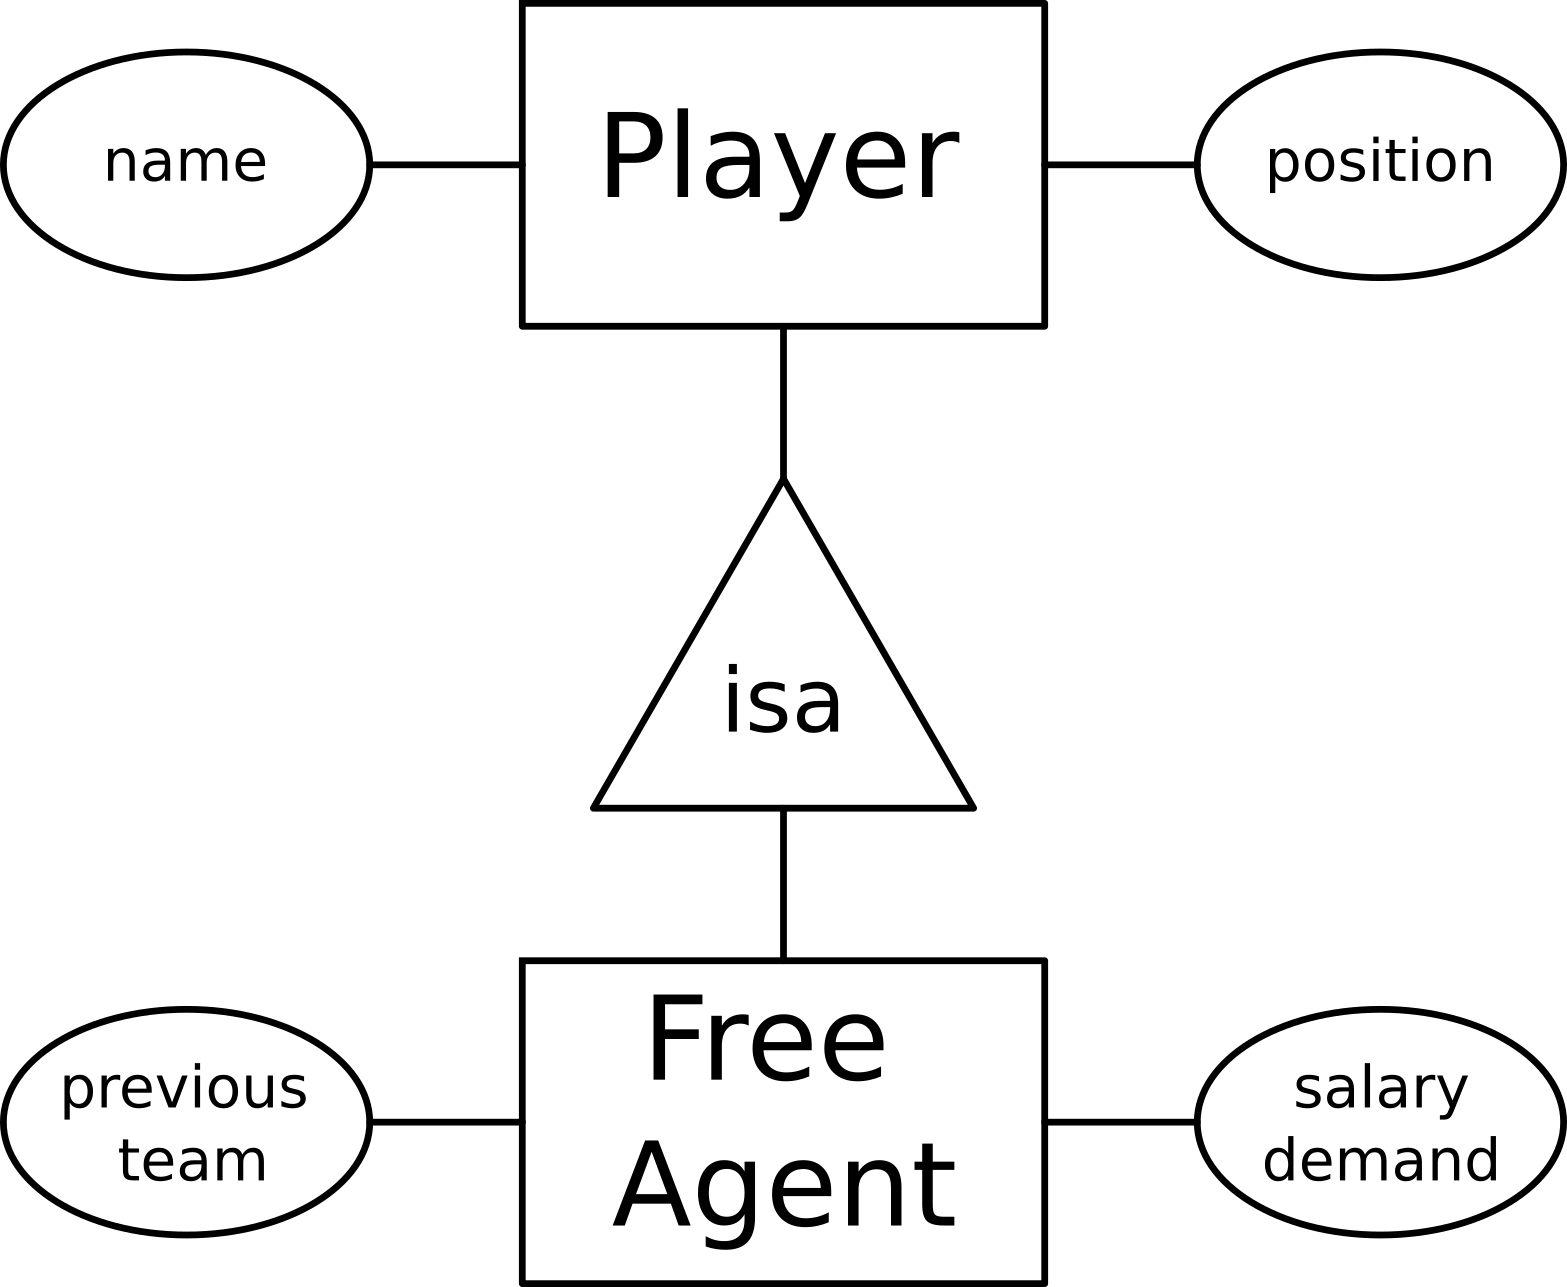
\includegraphics[width=0.3\linewidth]{entity12.png}
\end{figure}
\item There are multiple ways to implement subclasses:
\begin{enumerate}[label=(\roman*)]
\item Nulls: Use one relation with all possible attributes, and enter \lstinline|NULL| for inapplicable attributes.
\item Object-Oriented: Use one relation per subset of subclasses, each with all relevant attributes. Only list an object in one relation.
\item E/R-Style: Use one relation for each subclass with attributes of that subclass and key attributes. List an object in the subclass relation and all superclass relations.
\end{enumerate}
\item The E/R-Style is generally preferred, but it requires more complicated queries with joins

\begin{minipage}{0.25\linewidth}
\begin{figure}[H]
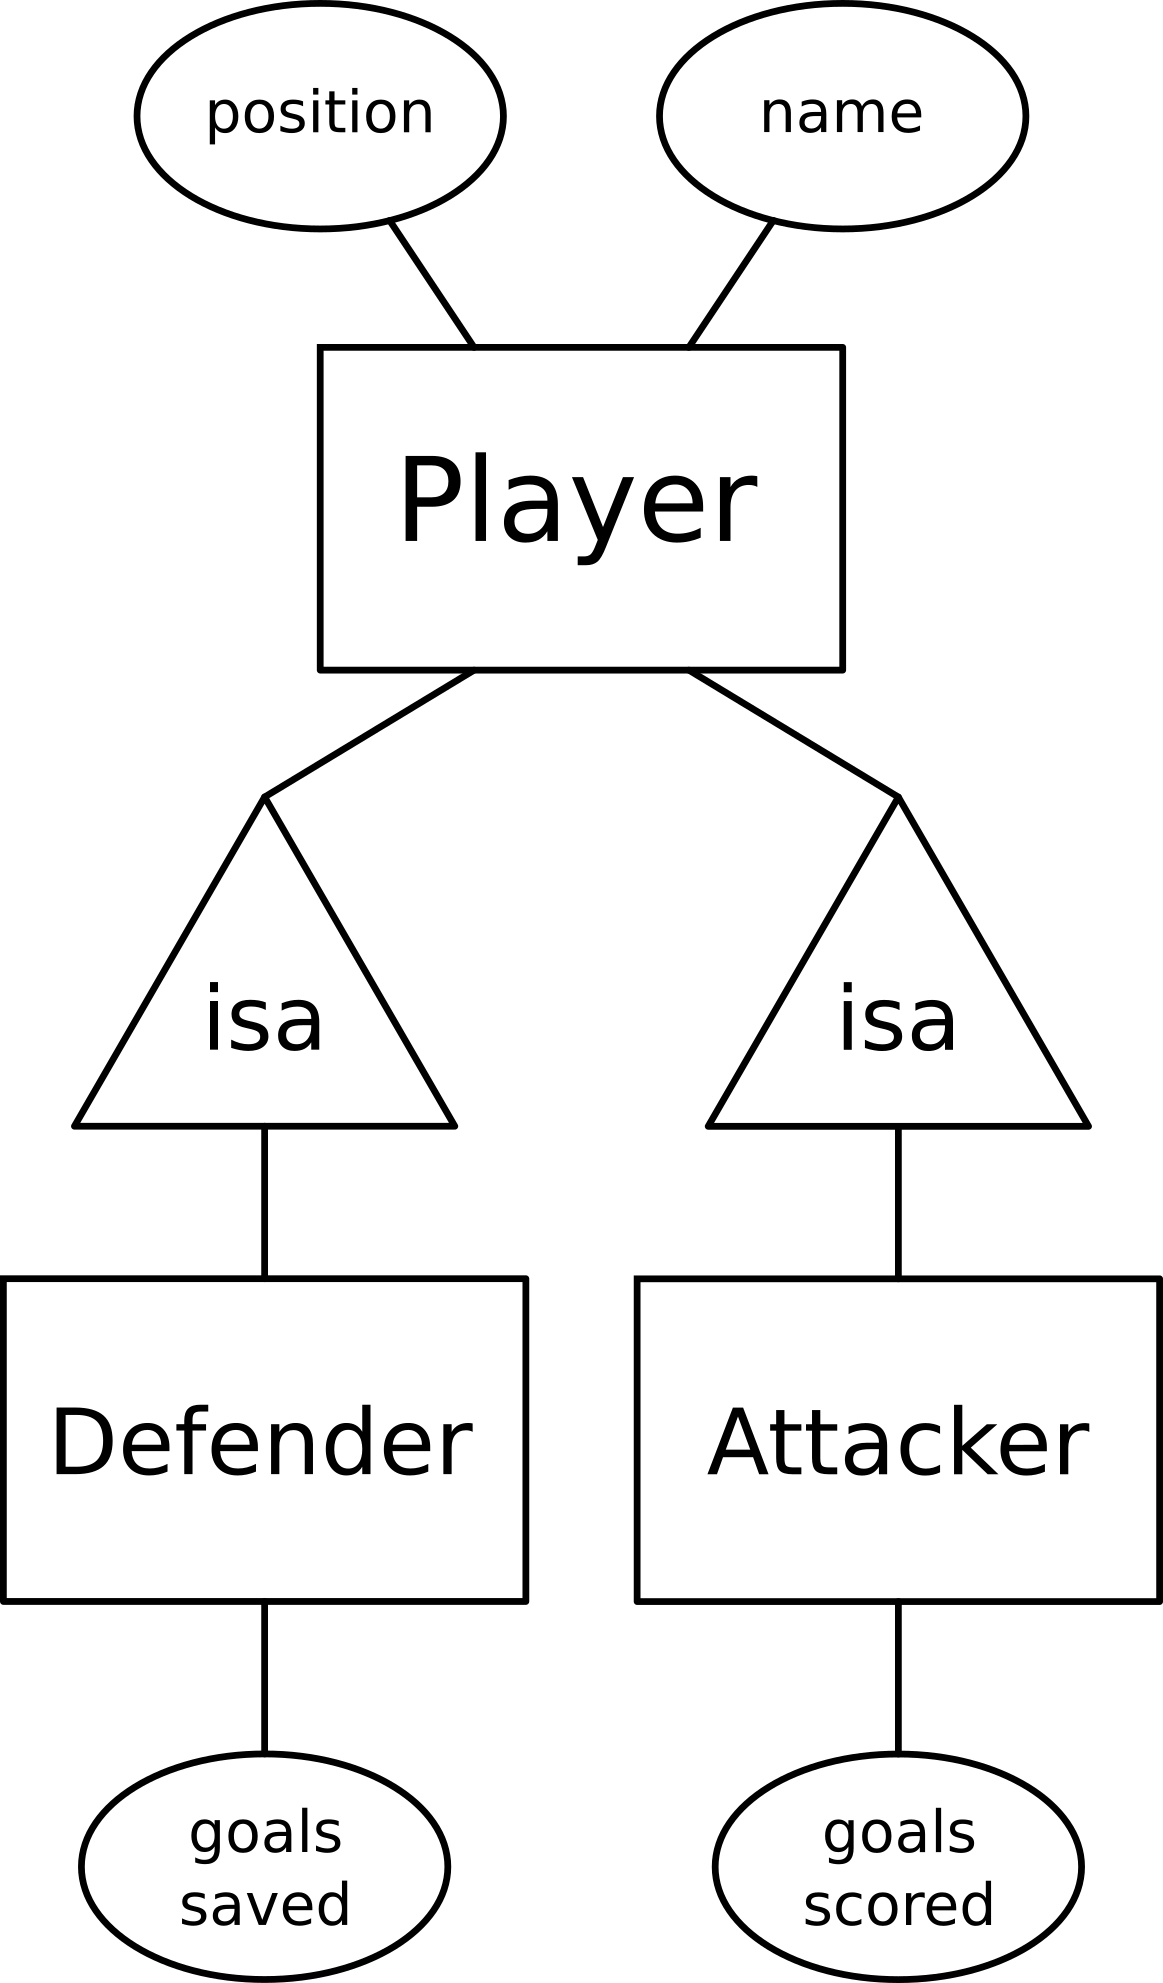
\includegraphics[width=\linewidth]{entity15.png}
\end{figure}
\end{minipage}
\hfill
\begin{minipage}{0.7\linewidth}
\begin{figure}[H]
\begin{subfigure}{\linewidth}
\centering
\begin{tabular}{llll}
\multicolumn{4}{c}{player}\\\toprule
name&position&saved&scored\\\midrule
Jimmy&Midfield&2&4\\
Jane&Defense&7&NULL\\
Jessica&Attack&NULL&14\\
Justin&Bench&NULL&NULL\\\bottomrule
\end{tabular}
\caption*{Null Method}
\end{subfigure}

\vspace{2em}

\begin{subfigure}{\linewidth}
\centering
\begin{tabular}{ll}
\multicolumn{2}{c}{player}\\\toprule
name&position\\\midrule
Justin&Bench\\\bottomrule
\end{tabular}
\hfill
\begin{tabular}{llll}
\multicolumn{4}{c}{attacker and defender}\\\toprule
name&position&saved&scored\\\midrule
Jimmy&Midfield&2&4\\\bottomrule
\end{tabular}
\\
\vspace{1em}
\begin{tabular}{lll}
\multicolumn{3}{c}{attacker}\\\toprule
name&position&scored\\\midrule
Jessica&Attack&14\\\bottomrule
\end{tabular}
\hfill
\begin{tabular}{lll}
\multicolumn{3}{c}{defender}\\\toprule
name&position&saved\\\midrule
Jane&Defense&7\\\bottomrule
\end{tabular}
\caption*{Object-Oriented Method}
\end{subfigure}

\vspace{2em}

\begin{subfigure}{\linewidth}
\centering
\begin{tabular}{ll}
\multicolumn{2}{c}{player}\\\toprule
name&position\\\midrule
Jimmy&Midfield\\
Jane&Defense\\
Jessica&Attack\\
Justin&Bench\\\bottomrule
\end{tabular}
\hfill
\begin{tabular}{ll}
\multicolumn{2}{c}{defender}\\\toprule
name&saved\\\midrule
Jane&7\\
Jimmy&2\\\bottomrule
\end{tabular}
\hfill
\begin{tabular}{ll}
\multicolumn{2}{c}{attacker}\\\toprule
name&scored\\\midrule
Jessica&14\\
Jimmy&4\\\bottomrule
\end{tabular}
\caption*{E/R-Style}
\end{subfigure}
\end{figure}
\end{minipage}
\end{itemize}

\subsection{Keys}
\begin{itemize}
\item A \emph{key} is a set of attributes for one entity set so that no two entities agree on all attributes in the key
\begin{arrows}
\item The key uniquely identifies each entity in the entity set
\item Every entity set must have a key, which is denoted with an underline
\item In a ``isa'' hierarchy, only the root entity set has a key, which must work for all subclasses
\end{arrows}
\begin{figure}[H]
\centering
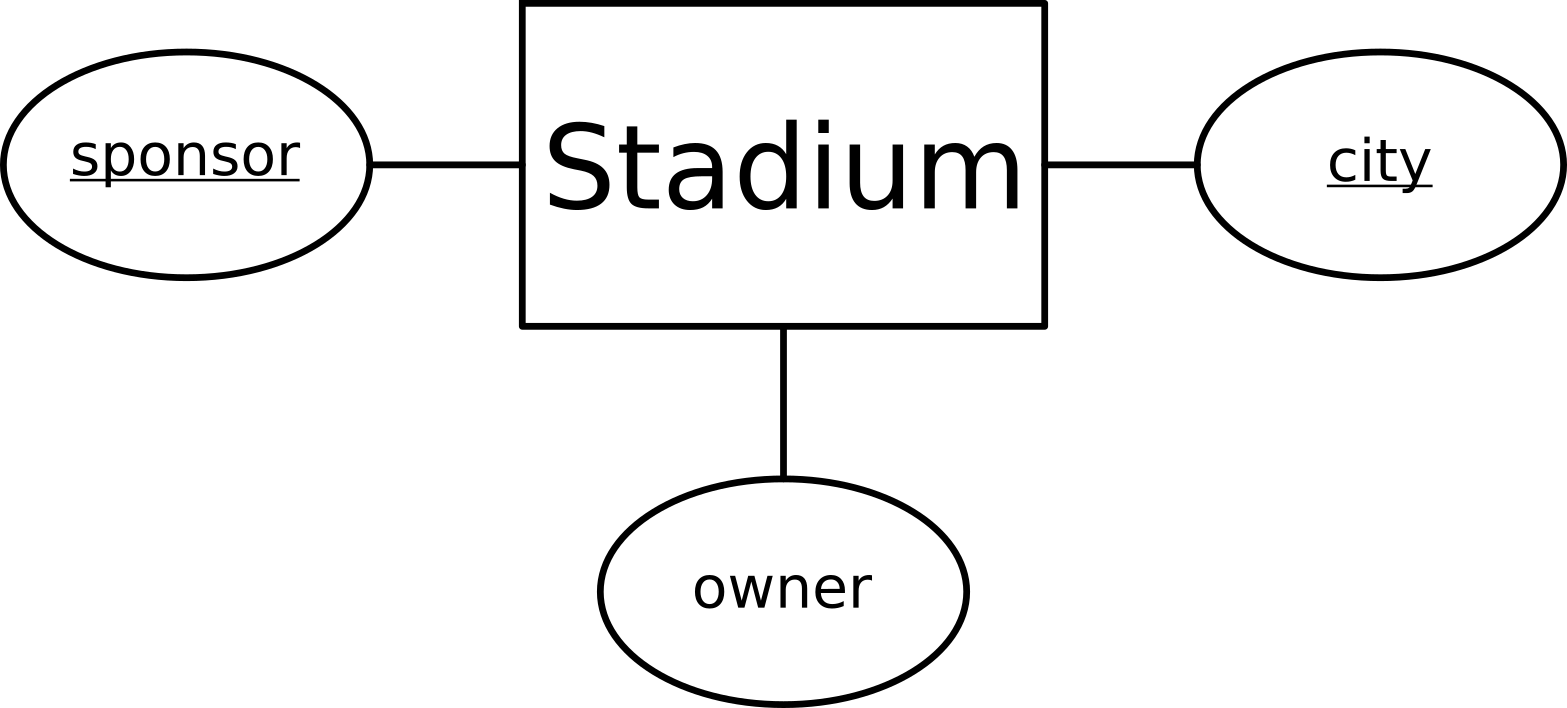
\includegraphics[width=0.3\linewidth]{entity13.png}
\end{figure}
\item A \emph{weak} entity $E$ is one such that the key of other entity sets needs to be included in order to uniquely identify entries, by following at least one many-to-exactly-one relationship from $E$
\begin{arrows}
\item This is denoted by adding a double outline around the weak identity and supporting relationships
\end{arrows}
\begin{figure}[H]
\centering
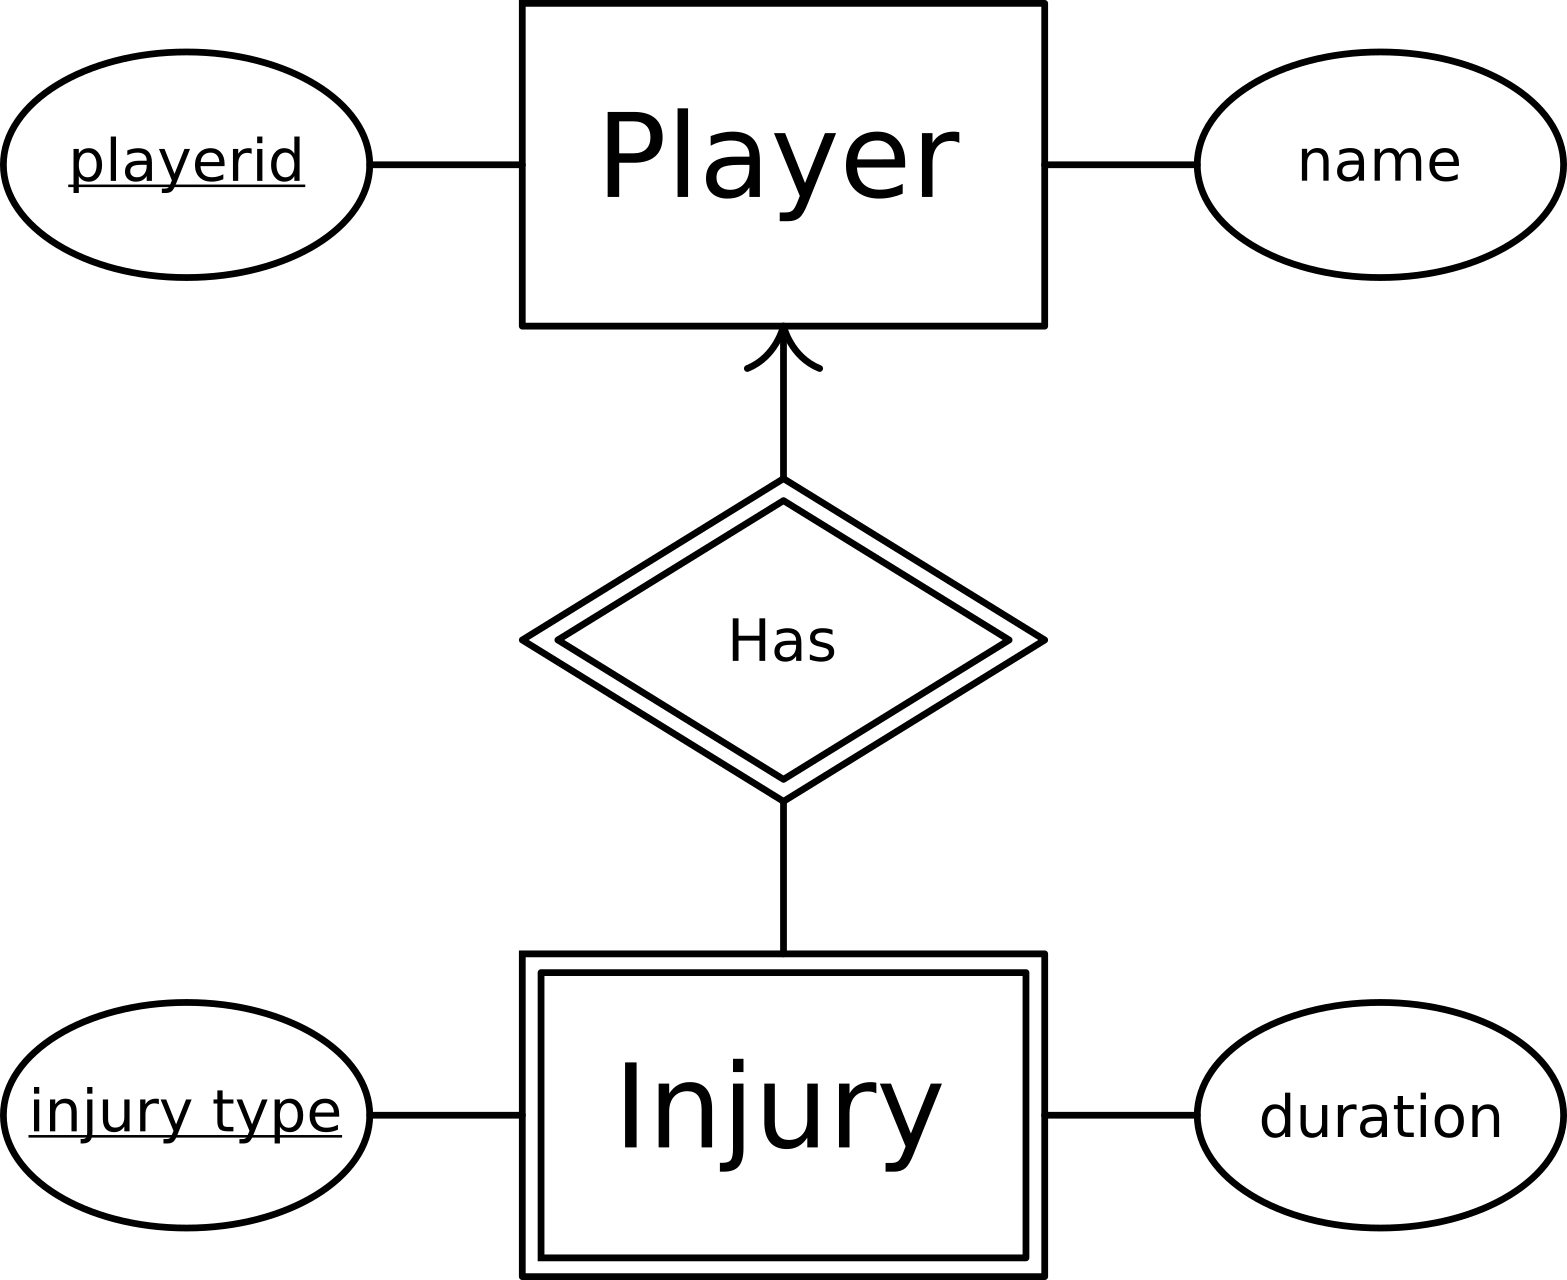
\includegraphics[width=0.3\linewidth]{entity14.png}
\end{figure}
\end{itemize}

\subsection{Design Decisions}
\begin{itemize}
\item Consider all the data in a database stored in a single table, with null values and redundancy. \emph{Decompositions} of this table are made when it is divided into smaller relations/entity sets. All decompositions should be \emph{lossless}, so that the original table could be recovered via natural joins on the subrelations
\item A database should avoid redundancy, both to limit space requirements and to reduce the risk of inconsistency
\begin{arrows}
\item Redundancy can occur when not enough decompositions are specified, i.e., the relations contain too much information and should be split into separate entity sets
\item This can lead to \emph{anomalies}, which are problems that occur specifically when too much information is contained a single relation
\item \emph{Update anomalies} occur when redundant information is updated in one location but not in other locations
\item \emph{Deletion anomalies} occur when a deletion causes more information to be deleted than desired (for example, deleting information about a group project when a single member of the group drops the class)
\end{arrows}
\begin{figure}[H]
\centering
\begin{subfigure}{0.39\linewidth}
\centering
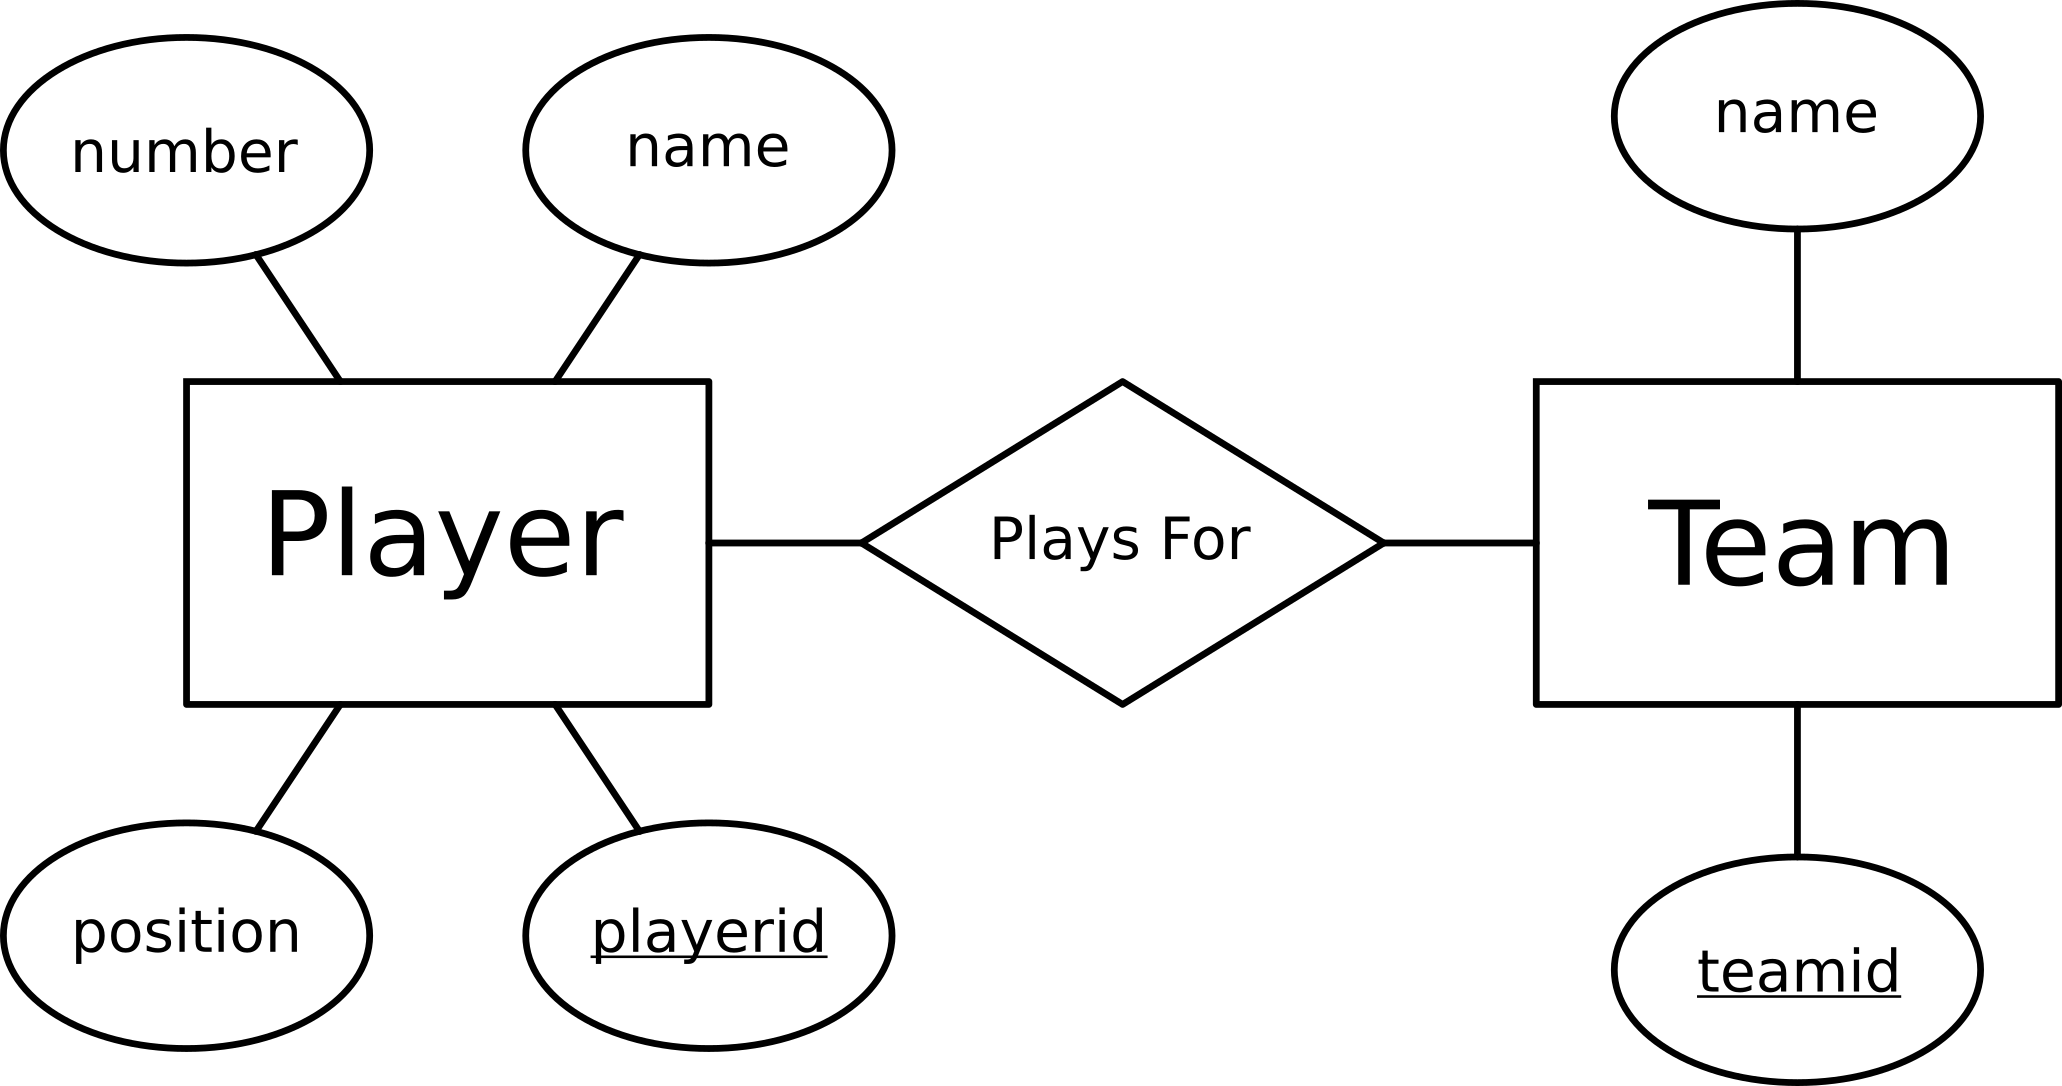
\includegraphics[width=0.9\linewidth]{entity16.png}
\caption*{Good Example}
\end{subfigure}
\begin{subfigure}{0.39\linewidth}
\centering
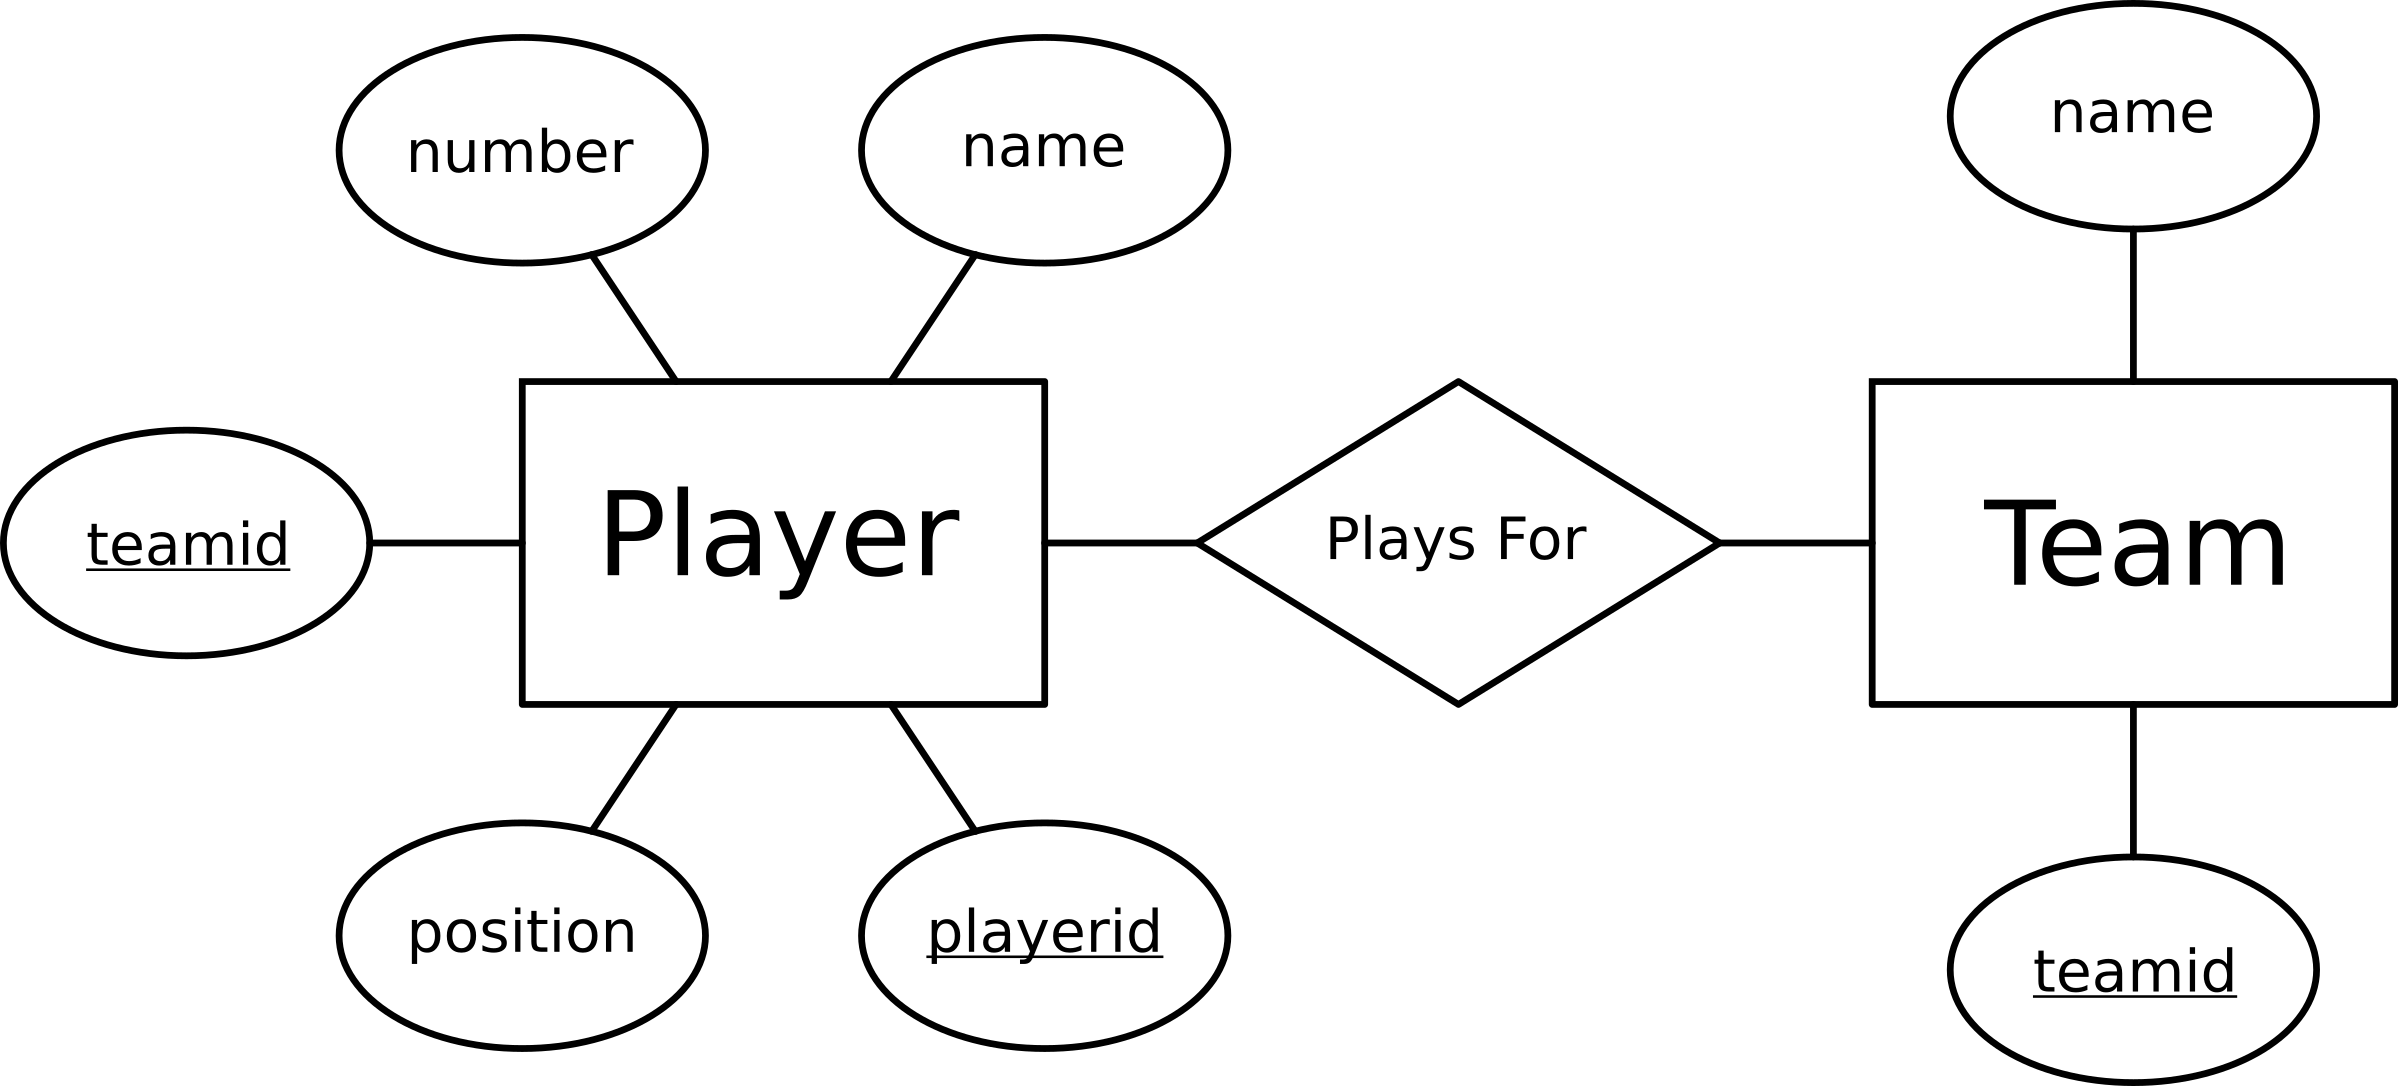
\includegraphics[width=0.9\linewidth]{entity17.png}
\caption*{Bad Example}
\end{subfigure}
\begin{subfigure}{0.19\linewidth}
\centering
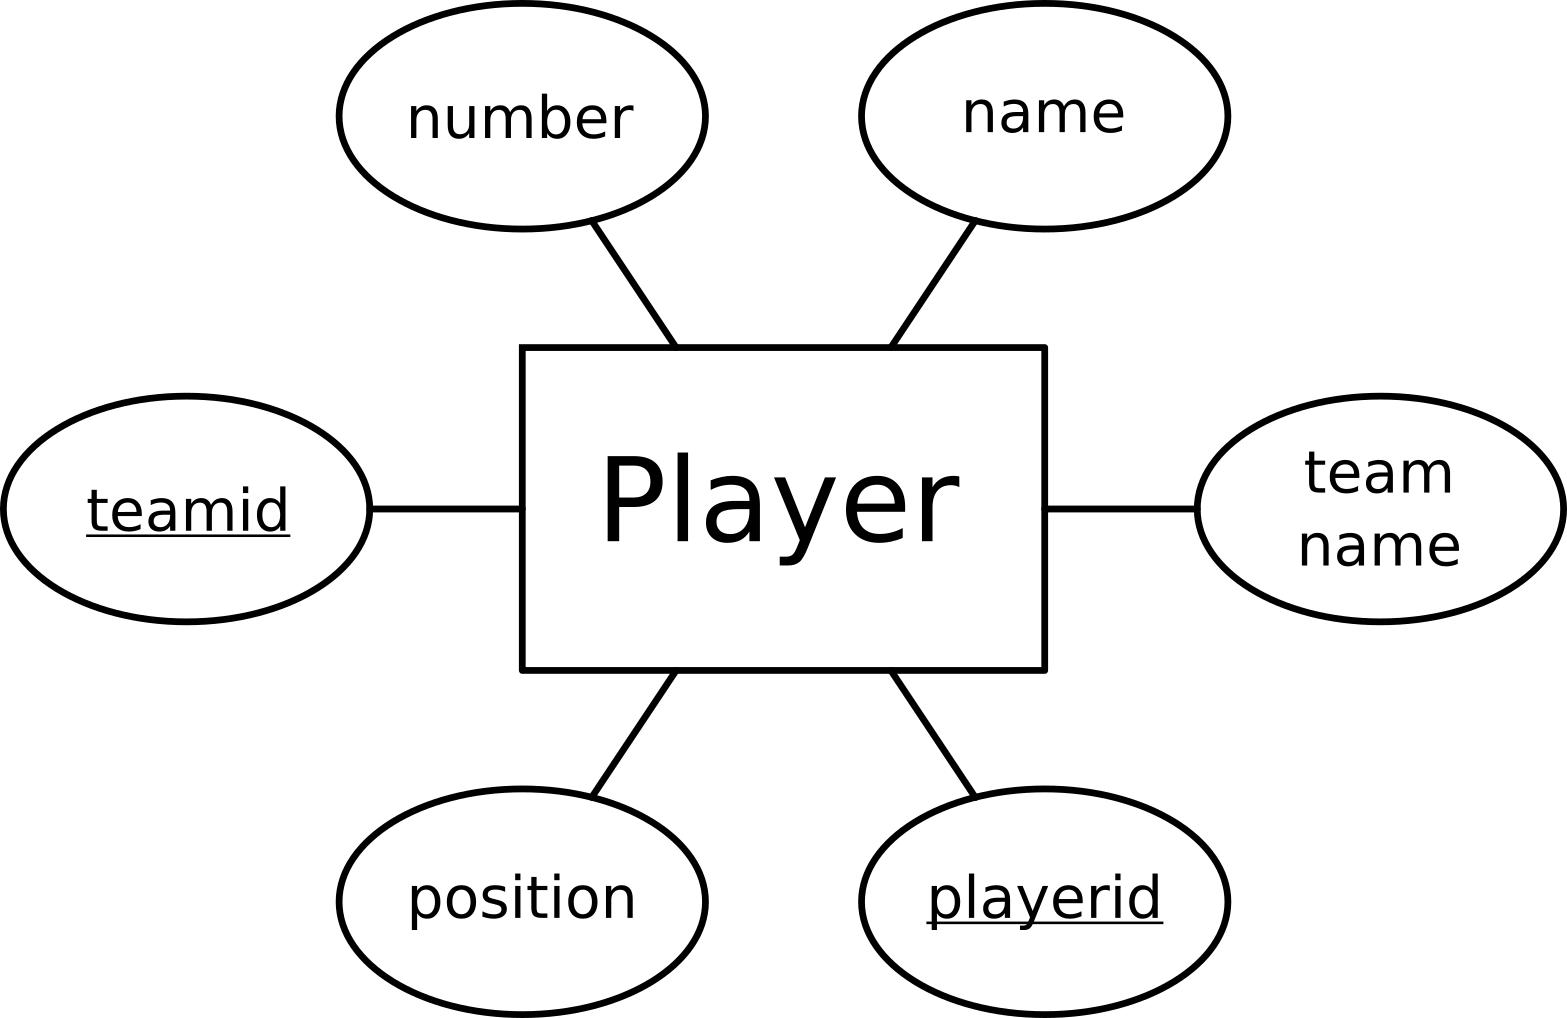
\includegraphics[width=0.9\linewidth]{entity18.png}
\caption*{Bad Example}
\end{subfigure}
\end{figure}
\item An entity set should be used instead of an attribute only when either:
\begin{enumerate}[label=(\roman*)]
\item The quantity is more than just the name of something; it has at least one non-key attribute
\item The quantity is the ``many'' part in a ``many-to-one'' or ``many-to-many'' relationship
\end{enumerate}
\begin{arrows}
\item For example, even if player only had one attribute, it would need to be an entity set since many players belong to a team
\item If team only had a single attribute, it should be an attribute of player rather than an entity set
\end{arrows}
\item Weak entities should not be overused
\begin{arrows}
\item It is better to create unique IDs for entity sets (e.g., social security numbers, automobile VINs, etc.
\item Weak entities are only needed when there is no global authority capable of establishing a unique identifier
\end{arrows}
\end{itemize}

\subsection{Converting E/R Diagrams to Relations}
\begin{itemize}
\item When converting an E/R diagram to relations/tables, each entity set becomes a relation with the corresponding attributes,
\item Each relationship becomes a relation whose attributes are:
\begin{enumerate}[label=(\roman*)]
\item The keys of the connected entity sets
\item Any attributes of the relationship itself
\end{enumerate}
\item In a many-to-one relationship, the table for the relationship can be combined with the ``many'' table

\begin{figure}[H]
\centering
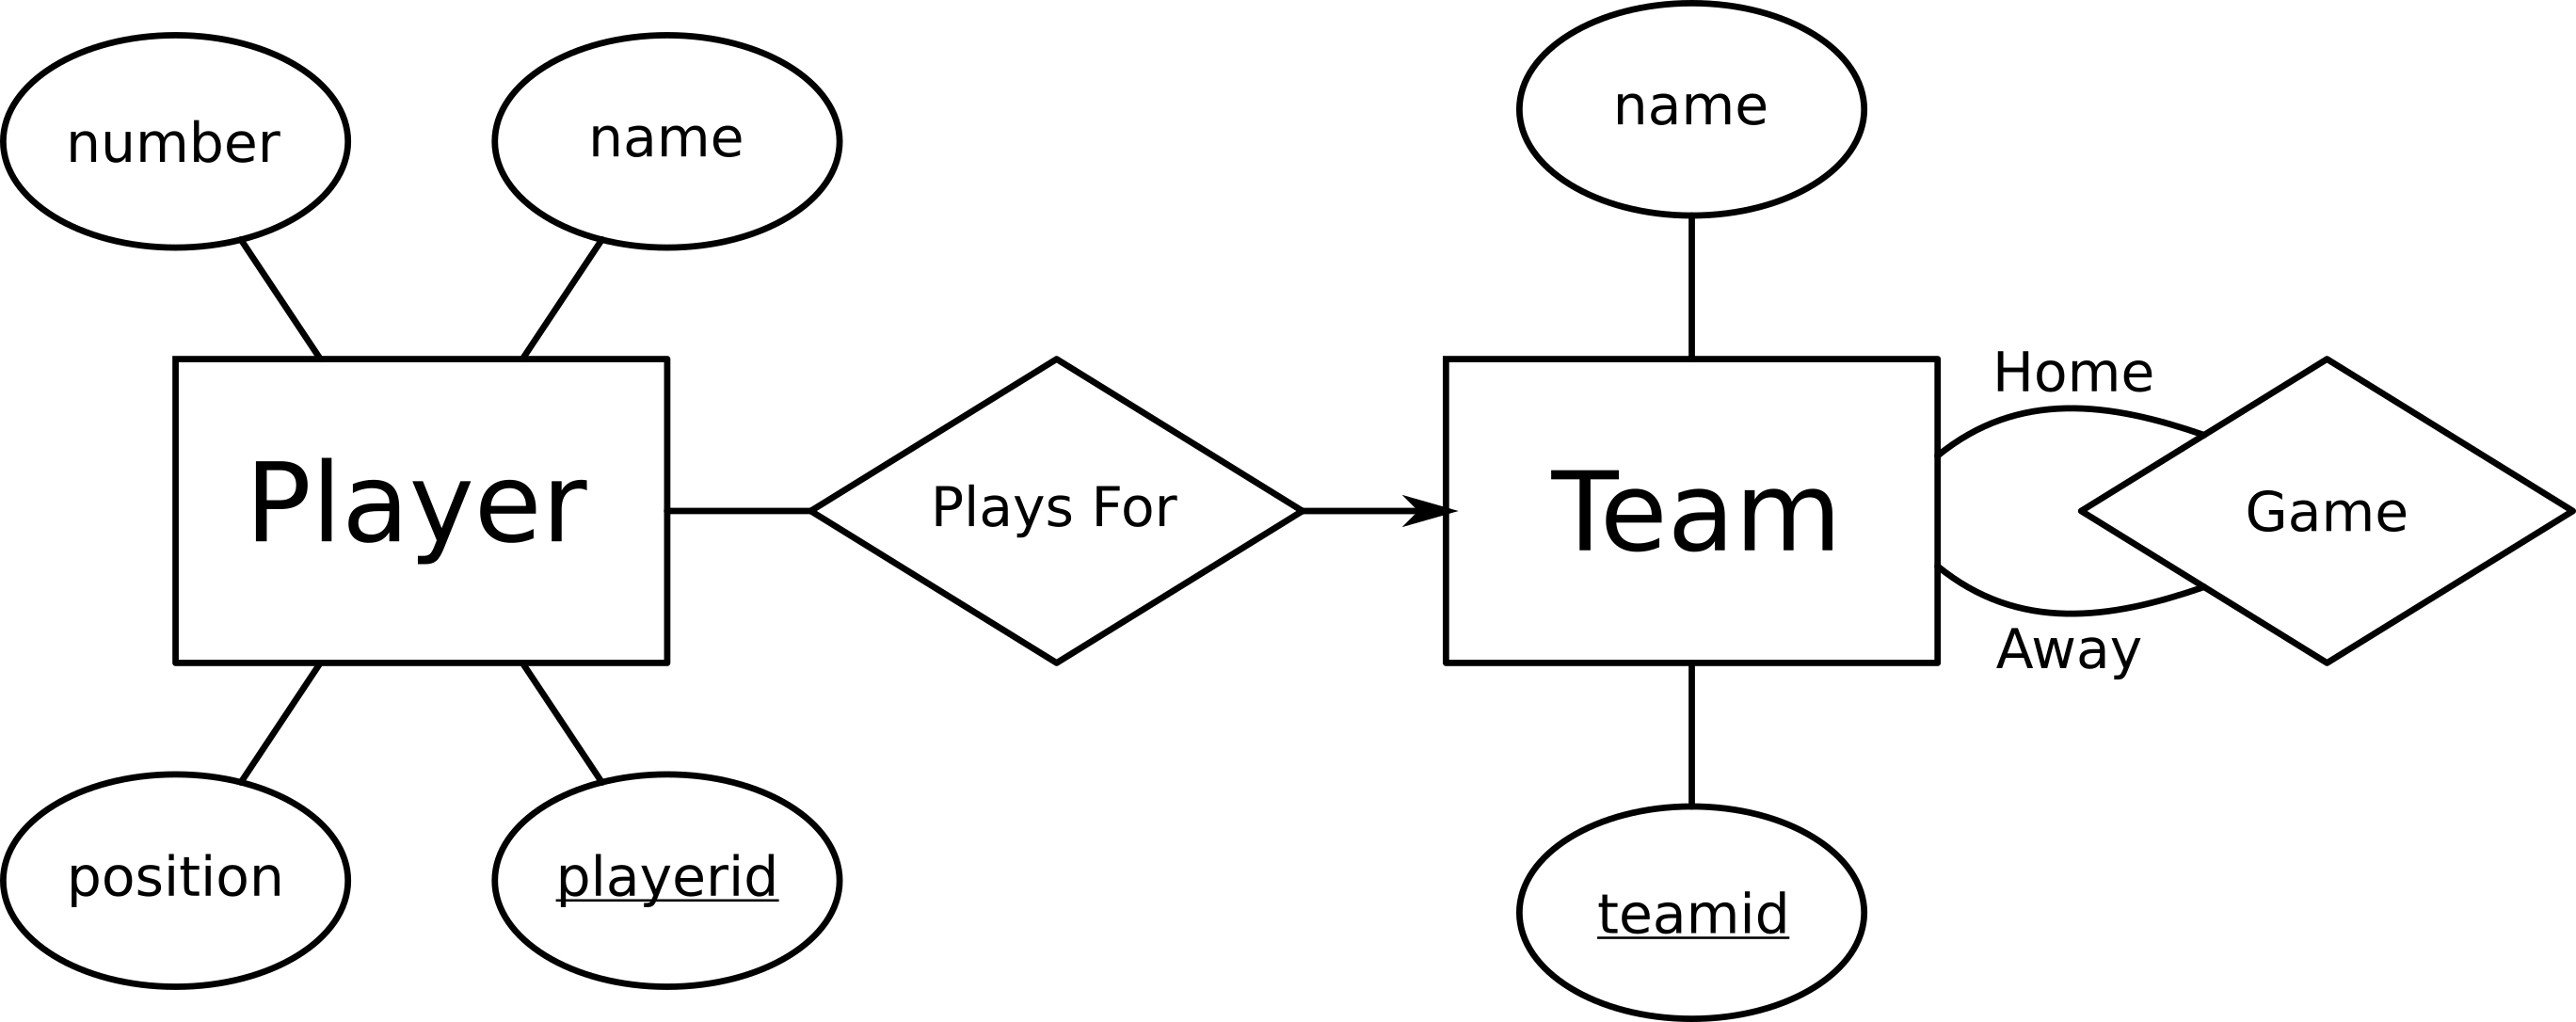
\includegraphics[width=0.7\linewidth]{entity19.png}\\
\vspace{1em}

\begin{minipage}{0.8\linewidth}
\raggedright
Relations:
\begin{itemize}
\item \lstinline|Player(playerid, name, number, position, teamid)|
\begin{arrows}
\item This is the result of merging \lstinline|Player(playerid, name, number, position)| and \lstinline|PlaysFor(playerid, teamid)|
\end{arrows}
\item \lstinline|Team(teamid, name)|
\item \lstinline|Game(home, away)|
\end{itemize}
\end{minipage}
\end{figure}
\end{itemize}


\section{Transaction Management}
\subsection{Introduction}
\begin{itemize}
    \item A \emph{transaction} is a unit of program execution that accesses and possibly updates various data items
    \item The principles of transactions for relational databases are summarized with then acronym \emph{ACID} (called the \emph{ACID Properties)}:
    \begin{itemize}
        \item[A:] \emph{Atomicity}. Despite consisting of possibly many statements, the collection must appear to the user as an indivisible unit: it either executes in entirety or not at all (if failure occurs for any reason, any changes must be undone)
        \item[C:] \emph{Consistency}. The database must remain in a consistent after an isolated transaction is run (data still is valid)
        \item[I:] \emph{Isolation}. Since transactions consist of many statements, it must be ensured that each transaction is not affected by other concurrent transactions
        \item[D:] \emph{Durability}. Successful transactions must remain permanent even if the system later crashes.
    \end{itemize}
    \item The primary way to make a database system more efficient is to allow for concurrency, but the scheduling of transactions cannot violate the ACID test; it must appear to the end-user that each query runs independently
    \begin{arrows}
        \item Note that no restrictions are placed on the order in which transactions are executed; if an order is required, they should be packaged in the same transaction
        \item All transactions must conform to the ``Correctness Principle'': if a transaction executes independently without system errors, and the database begins in a consistent state, then it must end in a consistent state
        \item When determining how to implement concurrency, there is a tradeoff between latency (wait-time for a given query) and throughput (the number of queries that can be processed at once)
    \end{arrows}
\end{itemize}
\subsection{Serializable Schedules}
\begin{itemize}
    \item A schedule is a \emph{serial schedule} if the actions consist of all the actions from one transaction, then all the actions of another transaction, and so on
    \item A schedule is a \emph{serializable schedule} if there exists a serial schedule producing the same output
    \begin{arrows}
    \item Serializable schedules may have actions being interweaved between transactions, resulting in concurrency, but it appears to the end user as if each runs in isolation
    \item A non-serializable schedule violates ACID properties, so may not be used by the database scheduler
    \end{arrows}
    \item When determining whether a schedule is serializable, only the details of what element is being written to/read from is used, not the actual contents of the read/write
    \begin{arrows}
    \item This means arithmetic coincidence cannot be utilized; for example, properties such as commutativity and associativity cannot be utilized
    \item The reason for this is understanding the effect of a query on the database is a hard problem, related to the Halting Problem
    \end{arrows}
\end{itemize}

\subsection{Conflict-Serializable Schedules}
\begin{itemize}
    \item A \emph{conflict} is a pair of consecutive actions in a schedule such that the output may change if their order is interchanged
    \begin{arrows}
        \item To identify conflicts (again assuming no arithmetic coincidence), we notate the operations as $r_i(X)$ and $w_i(X)$ for read and write, where $i$ is the transaction and $X$ is the database element
        \item Note that a write represents a \emph{blind write}, where the element is written to without being read (i.e., the element is overwritten)
    \end{arrows}
    \item Consider two actions $a_i(X)$ and $b_j(Y)$. We have:
    \begin{enumerate}[label=(\roman*)]
        \item There is a conflict if $i=j$, since we never allow actions within the same transaction to be re-ordered
        \begin{arrows}
        \item Although a transaction is represented by $r_i$ and $w_i$, other database-independent actions are also being performed; for example, the information of a read can be processed in some way and then used in a write
        \item Thus, it is not feasible to consider re-ordering transactions under this framework
        \end{arrows}
        \item Otherwise, if $X\neq Y$, there is no conflict, since different database elements are being utilized
        \item Finally, if $X=Y$, then there is a conflict iff either $a$ or $b$ is a write action
    \end{enumerate}
    \item Two schedules are \emph{conflict-equivalent} if one can be transformed to the other via non-conflicting swaps of adjacent actions
    \item A schedule is \emph{conflict-serializable} if it is conflict equivalent to a serializable schedule
    \begin{arrows}
    \item Every conflict-serializable schedule is serializable
    \item Not every serializable schedule is conflict-serializable, such as $r_1(X); w_2(x); w_1(X); w_3(X)$. This is not conflict serializable since $w_2(X)$ and $w_1(X)$ conflict, but it is serializable since in any order, the result is over-written by $w_3(X)$
    \item In practice, it is difficult to determine whether a schedule is serializable, but it is much easier to determine whether it is conflict-serializable
    \end{arrows}
    \item Transaction $i$ ($T_i$) \emph{takes precedence} over transaction $j$ ($T_j$) in schedule $S$ if there are actions $A_1\in T_1$ and $A_2\in T_2$ such that $A_1$ precedes $A_2$, $A_1$ and $A_2$ involve the same data element, and at least one is a write
    \begin{itemize}
        \item Equivalently, $T_i$ has precedence over $T_j$ if there exists conflicting actions $A_1\in T_i$ and $A_2\in T_j$ such that $A_1$ precedes $A_2$
        \item This is denoted $T_1<T_2$
    \end{itemize}
    \item In a conflict-serializable schedule, $T_i<T_j$ must imply that $T_i$ precedes $T_j$ in the corresponding serial schedule
    \begin{arrows}
    \item Thus, by building a precedence graph (a directed graph with edges from $T_i$ to $T_j$ for each $T_i<T_j$), a schedule is conflict-serializable iff it is acyclic
    \item A conflict-equivalent serial schedule can then be found via topological sorting
    \end{arrows}
\end{itemize}

\subsection{Locks}
\begin{itemize}
    \item \emph{Locks} provide a mechanism for producing conflict-serializable schedules while still allowing concurrency; transactions request and release locks on different elements of the database
    \item Locks control transactions as follows:
    \begin{arrows}
    \item A transaction may only read or write to an element if it was previously granted a lock and has not released the lock yet
    \item Transactions must eventually release all locks
    \item No two transactions can concurrently have a lock on the same element
    \end{arrows}
    \item Locking an element is denoted $l_i(X)$, and releasing a lock is denoted $u_i(X)$
    \item Simply having locks is not enough to ensure conflict-serializable schedules, since each action could simply lock and then immediately unlock the element
    \item \emph{Two-Phase Locking (2PL)} guarantees that a legal schedule of consistent transactions is conflict-serializable by forcing all lock actions to precede all unlock actions
    \begin{arrows}
        \item The \emph{expanding phase} consists of the portion of the transaction where locks may be acquired, and the \emph{shrinking phase} consists of the portion where locks may be released
        \item This ensures that no other transactions may interfere with a given element until the transaction is completely finished with it
    \end{arrows}
    \item To produce the schedule, each transaction can greedily request resources/locks, and the scheduler will either grant these are deny them
\end{itemize}

\subsection{Types of Locks}
\begin{itemize}
\item If multiple transactions only read from an element without writing to it, then hypothetically these could run concurrently in any order
\item To allow this, locks are divided into two categories: \emph{shared locks} and \emph{exclusive locks}
\item A shared lock is used for reading, while an exclusive lock is used for reading and/or writing
\item Many shared locks can be granted simultaneously, but an exclusive lock can only be granted if it is the only locks
\item Shared lock requests are denoted $sl_i(X)$ and exclusive locks are denoted $xl_i(X)$
\item Thus, all of the rules become:
\begin{arrows}
\item Consistency of Transactions: In any transaction $T_i$, $r_i(X)$ must be preceded by $sl_i(X)$ or $xl_i(X)$, with no intervening $u_i(X)$; $w_i(X)$ must be preceded by $xl_i(X)$ with no intervening $u_i(X)$; and $sl_i(X)$ and $xl_i(X)$ must eventually be followed by $u_i(X)$
\item Two-Phase Locking of Transactions: No action $sl_i(X)$ or $xl_i(X)$ may be preceded by $u_i(Y)$ for any $Y$
\item Legality of Schedules: If $xl_i(X)$ appears in a schedule, then no $xl_j(X)$ or $sl_j(X)$ may appear for $j\neq i$ until $u_i(X)$ appears; and if $sl_i(X)$ appears in a schedule, then there cannot be a following $xl_j(X)$ for $j\neq i$ until $u_i(X)$ appears
\end{arrows}
\end{itemize}

\subsection{Transactions in SQLite}
\begin{itemize}
\item SQLite chooses to lock on the entire database at a time, rather than locking on a table/row/value
\begin{arrows}
\item This sacrifices efficiency for ease of implementation
\item Due to triggers, it may be difficult to determine how a given action impacts the database
\end{arrows}
\item There are five locking states of the database:
\begin{arrows}
\item \lstinline|UNLOCKED|. No locks are held on the database, and the database can not be read or written. This is the default state.
\item \lstinline|SHARED|. The database may be read but not written. Any number of processes can hold a shared lock, so many simultaneous reads can occur.
\item \lstinline|RESERVED|. A single process has a reserved lock, indicating that it plans to eventually write to the database, but that shared locks can continue being acquired until then.
\item \lstinline|PENDING|. A single process has a pending lock, indicating that it plans to write to the database as soon as possible. No new shared locks may be acquired, although existing shared locks are allowed to finish.
\item \lstinline|EXCLUSIVE|. A single process may have an exclusive lock, and no other locks may be present at that time. This lock permits reads and writes. Since this limits concurrency, SQLite minimizes the number of these locks granted.
\end{arrows}
\item A transaction in SQLite ends with either a commit, rollback, or error (which in turn triggers a rollback)
\begin{arrows}
\item These are denoted in a schedule with $\text{commit}_i$ and $\text{rollback}_i$
\item Typically, the transaction does not write to the database until the commit, and instead modifies a local cached copy (so that different transactions may see different snapshots of the database)
\item More formally, SQLite uses write-ahead logging (WAL) to record changes to the database (so a literal copy is not made, but this is an easy way to think about it)
\item It is possible that a write may occur sooner that the commit (perhaps when using the immediate/exclusive mode) %!!! CLARIFY ON PIAZZA
\item In the case of a rollback/error, all changes are undone
\item All locks are released upon commit
\end{arrows}
\item A transaction can be run in three modes:
\begin{arrows}
\item \lstinline|DEFERRED|. A shared lock is requested upon the first read, and an exclusive lock is requested upon the first write (recall that the write typically occurs on commit, not on the first update/insert statement). This is the default.
\item \lstinline|IMMEDIATE|. A reserved lock is requested immediately, and it will fail or wait if another transaction is holding an exclusive/reserved/pending lock. An exclusive lock is requested prior to writing (typically the promotion occurs on commit).
\item \lstinline|EXCLUSIVE|. An exclusive lock is requested immediately, and it will fail or wait if other locks are being held.
\end{arrows}
\item The syntax in SQLite is \lstinline|BEGIN [MODE] TRANSACTION| for beginning the transaction (where \lstinline|[MODE]| is optionally passed), and either \lstinline|COMMIT TRANSACTION| or \lstinline|ROLLBACK TRANSACTION|.
\item Statements executed outside of explicit transactions are handled differently depending on the \lstinline|isolation_level| property specified when forming the connection
\begin{arrows}
\item \ilpy{'DEFERRED'}, \ilpy{'IMMEDIATE'}, or \ilpy{'EXCLUSIVE'}. Transactions in these modes are implicitly opened in the respective mode before any \lstinline|INSERT|, \lstinline|UPDATE|, \lstinline|DELETE|, or \lstinline|REPLACE| statement is run. The transaction must be explicitly committed or rolled back with \ilpy{commit()} or \ilpy{rollback()}, otherwise the changes are rolled back. The default is \ilpy{'DEFERRED'}.
\item \ilpy{None}. Each executed statement is treated as its own transactions, automatically committed after it finishes. This mode is often better to use, since it is better to explicitly open transactions when they are needed.
\end{arrows}
\item If a statement cannot be run because it cannot acquire the locks, then SQLite issues an error after a certain amount of time
\end{itemize}

\subsection{Rollbacks}
\begin{itemize}
\item A \emph{rollback} aborts a transaction and undoes its changes (which is necessary by atomicity)
\item If a serial schedule is not used, rolling back one transaction may require that previous transactions be rolled back as well
\begin{arrows}
\item Namely, if a transaction $T_1$ has read modified (uncommitted) data created by $T_2$, then a rollback of $T_2$ also requires that $T_1$ be rolled back
\item This can lead to \emph{cascading rollbacks}
\item Cascading rollbacks can be avoided using \emph{strict two-phase locking}, which only allows locks to be released at the moment of commit or rollback, and not sooner
\item There is a tradeoff between throughput and preventing cascading rollbacks
\end{arrows}
\item Rollbacks can be handled %!!! FINISH, and discuss which way SQLite3 does it
\end{itemize}

\subsection{Deadlock}
\begin{itemize}
\item In a locking schedule, \emph{deadlock} occurs when transactions are waiting for locks to be released, but they are holding the locks that other transactions need to continue
\item Deadlock can be detected via a \emph{Wait-For graph}, where each transaction is a node, and directed edges point from the waiting transaction to the transaction it is waiting on
\begin{arrows}
\item If the Wait-For graph has a cycle, then there is deadlock
\item Deadlock must be resolved by rolling back a transaction
\item However, many methods do not directly detect deadlock via waits-for graphs, and instead impose other rules
%!!! Add picture/example
\end{arrows}
\item Using a timeout is one method of deadlock resolution, where any transaction waiting for some number of seconds is rolled back
\begin{arrows}
\item Choosing the threshold is difficult and may not solve the issue if the transactions are resubmitted the same way
\end{arrows}
\item The Wait-Die and Wound-Wait methods resolve deadlocks by rolling back transactions based on their timestamps when one transactions requests the resources/locks of another
\begin{arrows}
\item No explicit deadlock detection is performed; rather, the rules make it so that deadlock could not possibly occur
\item Each transaction $T_i$ is assigned a timestamp $ts(T_i)$ for when it starts, where $ts(T_i)<ts(T_j)$ indicates that $T_i$ is older (such as with Unix time)
\item Both methods give priority to older transactions, but in different ways
\item When a transaction is rolled back, then it restarts with the same timestamp, so that it will eventually be the oldest (being rolled back does not penalize its priority)
\item A waiting transaction tries to get the lock again as soon as it is free, but when a rolled back transaction resurfaces is less predictable
\end{arrows}
\item When $T_i$ requests a lock held by $T_j$, the \emph{Wait-Die} deadlock resolution method performs one of two actions:
\begin{arrows}
\item If $ts(T_i)<ts(T_j)$, $T_i$ waits for $T_j$ (older waits for younger)
\item Otherwise, $T_i$ aborts (younger dies)
\end{arrows}
%!!! Add example
\item Similarly, the \emph{Wound-Wait} deadlock resolution method takes the actions:
\begin{arrows}
\item If $ts(T_i)<ts(T_j)$, then $T_j$ aborts (older wounds younger, forcing it to roll back)
\item Otherwise, $T_i$ waits (younger waits for older)
\end{arrows}
\item Both these methods minimize \emph{starvation}, which is when objects are less efficient due to waiting for resources (deadlock is the most extreme form of this)
\begin{arrows}
\item Wait-Die tends to roll back more transactions than Wound-Wait (since all younger transactions die when requesting resources from older), but the transactions have done less work when they are rolled back
\end{arrows}
\item These methods do not specify when each transaction is allocated time to run its actions; one method is \emph{round-robin style scheduling}, which performs one action from each transaction in an alternating fashion
\begin{arrows}
\item Commit is treated as its own action
\item If a transaction is waiting on a lock, it can try again next time (but this means that younger transactions may acquire it sooner)
\end{arrows}
\end{itemize}

\subsection{Validation Scheduling}
\begin{itemize}
\item Locks are a form of \emph{pessimistic concurrency control} because they assume transactions will conflict unless the scheduler prevents them
\item \emph{Validation} is an optimistic way of ensuring serializable schedules, which assumes that conflicts are rare
\begin{arrows}
\item This is useful when most transactions are readers, and only small fractions of the total database are accessed/modified by any transaction
\end{arrows}
\item Each transaction has three phases:
\begin{arrows}
\item A read phase, where all writes occur to private storage
\item A validation phase, where it is checked that no conflicts will occur if the write phase happens
\item A write phase, where the writes are made public if the validation is successful (otherwise the transaction is aborted)
\end{arrows}
\item In particular, validation ensures that the schedule generalized will be equivalent to the serial schedule ordered by timestamp (all conflicts must occur in one direction)
\item The validation test for $T_j$ check that for all $ts(T_i)<ts(T_j)$, we have one of the following:
\begin{enumerate}[label=\arabic*.]
\item $T_i$ completes its write phase before $T_j$ starts its read phase
\begin{arrows}
\item This is what would occur in a serial schedule
\end{arrows}
\item ($T_i$ does not write to any object that $T_j$ reads from) and ($T_i$ completes its write phase before $T_j$ starts its write phase)
\begin{arrows}
\item Writes/reads from $T_i$ can be interweaved with reads of $T_j$ as long as there is no WR conflict
\item No writes are interweaved
\end{arrows}
\item ($T_i$ does not write to any object that $T_j$ reads from) and ($T_i$ does not write to the same element that $T_j$ writes to) and ($T_i$ completes its read phase before $T_j$ completes its read phase)
\begin{arrows}
\item Writes may now be interweaved as well, under the condition that writes in $T_i$ act on objects which $T_j$ does no interact with
\item To ensure $T_j$ (the later transaction) does not impact $T_i$ (the earlier transaction), we must have that $T_i$ completes its read phase before $T_j$ completes its write phase (i.e., $T_j$ cannot begin to write while $T_i$ is still reading, so that all conflicts are resolved as RW)
\end{arrows}
\end{enumerate}
\end{itemize}

\subsection{Timestamp-Based Scheduling}
\begin{itemize}
\item Timestamp-based scheduling is also optimistic, but validates each action as it occurs, rather than all at once in a validation phase
\item To accomplish this, every database element has the additional metadata:
\begin{arrows}
\item $RT(X)$: The \emph{read time} of $X$, which is the most recent time $X$ was read
\item $WT(X)$: The \emph{write time} of $X$, which is the most recent time $X$ was written to
\item $C(X)$: The \emph{commit bit} of $X$, which is a boolean for whether the most recent write to $X$ has been committed
\end{arrows}
\item \emph{Physically unrealizable behaviors} are those that yield results incapable of being produced by the serial schedule where each transaction runs in order according to its start time
\begin{arrows}
\item This method aims to prevent these behaviors
\item For $T_i$ beginning before $T_j$, \emph{read-too-late} occurs when $r_i(X)$ occurs after $w_j(X)$, and \emph{write-too-late} occurs when $w_i(X)$ occurs after $r_j(X)$
\item These are essentially the conflicts from before, aside from write-write conflicts - in this case, $T_i$ can just skip its write action by the following rule
\end{arrows}
\item The \emph{Thomas Write Rule} states that write may be skipped if a later write is in place
\begin{arrows}
\item The one exception is when the later write is aborted (in which case the earlier write should have occurred)
\item In this case, these writes are ``delayed'' until either the later transaction is committed (in which case they do not run) or aborted (in which case they do run). This is kept track of with the committed bit
\end{arrows}
\item The rules for a transaction $T_i$ doing a read $r_i(X)$ are:
\begin{enumerate}
\item If $ts(T_i)>WT(X)$, then the read is physically realizable, so:
\begin{enumerate}[label=(\roman*)]
\item If $C(X)$ is true, then perform $r_i(X)$ and update $RT(X)=\max\{ts(T_1),RT(X)\}$
\item If $C(X)$ is false, then delay $r_i(X)$ until the transaction which wrote to $X$ commits or aborts
\end{enumerate}
\item If $ts(T_i)<WT(X)$, then the read is physically unrealizable (read-too-late), so roll back and restart with a new timestamp
\end{enumerate}
\item The rules for a transaction $T_i$ doing a write $w_i(X)$ are:
\begin{enumerate}
\item If $ts(T_i)>RT(X)$ and $ts(T_i)>WT(X)$, then it is physically realizable, so store a copy of $X$ in case of rollback, perform $w_i(X)$, and set $WT(X)=ts(T_i)$ and $C(X)$ to false
\item If $ts(T_i)>RT(X)$ and $ts(T_i)<WT(X)$, then it is physically realizable but has already been written to, so:
\begin{enumerate}[label=(\roman*)]
\item If $C(X)$ is true, then the Thomas Write Rule applies, so do nothing
\item If $C(X)$ is false, then delay the action until the other transactions commits or aborts
\end{enumerate}
\item If $ts(T_i)<RT(X)$, then the write is physically unrealizable (write-too-late), so roll back and restart with a new timestamp
\end{enumerate}
\item When $T_i$ commits, it finds all of the elements it wrote to and sets the commit bits to true
\item When $T_i$ rolls back, restore the old values of any elements written to, and allow the waiting transactions to perform reads/writes
\end{itemize}

\subsection{Comparison of Concurrency Control Methods}
\begin{itemize}
\item For the optimistic methods, validation and timestamp-based methods have similar performance and rates of rollback
\begin{itemize}
\item Validation has overhead all at once during the validation phase, while timestamp methods have overhead distributed across all actions
\end{itemize}
\item Storage requirements for locking and validation methods are similar
\begin{arrows}
\item Locking has storage requirements proportional to the number of elements locked
\item Validation needs to store timestamps and the sets of elements accessed/modified for all open transactions
\end{arrows}
\item Locking has few rollbacks, while validation has more frequent rollbacks
\item Validation has fewer delays in transactions, while locking can cause delays due to starvation
\end{itemize}

\section{Relational Database Model}
\subsection{Structure of Relational Databases}
\begin{itemize}
    \item A relational database stores data in tables, called \emph{relations}
    \begin{arrows}
        \item The rows of a relation are called \emph{tuples}
        \item The columns of a relation are called \emph{attributes}
        \item The relation may be given a name
    \end{arrows}
    \item A relation may have a \emph{relation schema}, which consists of a name for the relation and a list of its attributes, optionally with their corresponding \emph{domains}, or sets of possible values
    \begin{arrows}
        \item The database is therefore the collection of all relations, whereas the database schema is the collection of all relation schemas
    \end{arrows}
\end{itemize}

\section{SQL}
\subsection{Introduction to SQL}
\begin{itemize}
    \item Databases typically use restricted languages such as SQL
    \begin{arrows}
        \item This is easier to optimize and faster to write
        \item Often they are not Turing-complete, although technically SQL is
    \end{arrows}
    \item SQL offers both querying and a component for data-definition (describing database schemas)
    \item SQLite is a database engine which can be used in Python
    \item SQL statements fall into two categories:
    \begin{arrows}
        \item \emph{Data Definition Language (DDL)}, which build/modify the structure of the tables/objects, including \ilsql{CREATE}, \ilsql{ALTER}, and \ilsql{DROP}
        \item \emph{Data Manipulation Language (DML)}, including adding/removing/querying data
        \item DML is often summarized by the acronym \emph{CRUD}: create, read, update, and delete
    \end{arrows}
\end{itemize}

\subsection{SQL Style}
\begin{itemize}
    \item Semicolons should terminate each statement
    \item SQL keywords should be in all capitals
    \item Whitespace is only relevant in strings, although good practices are shown in the examples below
\end{itemize}

\subsection{SQLite Datatypes}
\begin{itemize}
    \item SQLite offers the following datatypes:
    \begin{itemize}
        \item \ilsql{INTEGER}, a signed integer up to 8 bytes long
        \item \ilsql{REAL}, a signed float using decimal or exponential notation (using capital E)
        \item \ilsql{TEXT}, a string of any length delimited by single quotes
        \begin{arrows}
            \item Single quotes are escaped by including two of them
            \item Other databases limit the length of strings, but SQLite does not
        \end{arrows}
        \item \ilsql{BLOB}, used to hold arbitrary binary data, such as images or videos
        \begin{arrows}
            \item This has no storage limits, although storing file paths is often easier
        \end{arrows}
    \end{itemize}
    \item Any datatype may also be \ilsql{NULL}
    \begin{arrows}
        \item It is used to represent an absence of information or an inapplicable value
        \item It should not be used to represent empty strings, false, or 0
    \end{arrows}
    \item Dates and times can be represented as \ilsql{TEXT} (ISO8601 strings, \texttt{"YYYY-MM-DD HH:MM:SS.SSS"}), \ilsql{REAL} (Julian day numbers), or \ilsql{INTEGER} (Unix time)
    \item Other types not in SQLite include Memo (65536 characters), Currency (15 whole digits and 4 decimal places), Yes/No (Microsoft Access), and Enum
    \item One way of working with other types in SQLite is to use adapters/converters
    \begin{arrows}
        \item An adapter is a function for converting a Python object into one of SQL's supported types, and is registered with \ilpy{sqlite3.register_adapter(python_type, adapter)}
        \item A converter is a function converting a \ilpy{bytes} object back into a desired Python object, and is registered with \ilpy{sqlite3.register_converter(sql_name, converter)}
        \item Note that these are registered with the module, not the connection
        \item To instruct SQLite to convert custom types during insertion, pass \ilpy{detect_types=sqlite3.PARSE_DECLTYPES} when forming the connection
        \item To apply converter upon selection, use \ilsql{SELECT col AS "col [type]" FROM table;} and specify \ilpy{detect_types=sqlite3.PARSE_COLNAMES} when forming the connection
        \item Both options can be specified by using \ilpy{detect_types=sqlite3.PARSE_DECLTYPES | sqlite3.PARSE_COLNAMES}
    \end{arrows}
\begin{python}
def adapt_color(color):
    return f"{color.r};{color.g};{color.b}"
def convert_color(bytestring):
    as_str = bytestring.decode("ascii")
    r, g, b = [float(x) for x in as_str.split(';')]
    return Color(r,g,b)
sqlite3.register_adapter(Color, adapt_color)
sqlite3.register_converter("COLOR", convert_color)
c = Color(24, 69, 59)
conn = sqlite3.connect(":memory:", detect_types = sqlite3.PARSE_DECLTYPES | sqlite3.PARSE_COLNAMES)
conn.execute("CREATE TABLE my_colors (col COLOR);")
conn.execute("INSERT INTO my_colors VALUES (?);", c)
res = conn.execute('SELECT col AS "col [COLOR]" FROM my_colors;')
row = next(res)
\end{python}
\end{itemize}

\subsection{Adding Data}
\begin{itemize}
    \item A relation is created via the \ilsql{CREATE TABLE} statement:
\begin{sql}
CREATE TABLE table_name (
    column1 datatype,
    column2 datatype,
    column3 datatype
);
\end{sql}
    \item The datatypes are optional, and are not enforced by SQLite
    \item A relation can be created from another table/query by:
    \begin{sql}
CREATE TABLE new_table AS
SELECT column1, column2
FROM old_table
\end{sql}
\item Tuples are added to the table via the \ilsql{INSERT INTO} statement:
    \begin{sql}
INSERT INTO table_name (column1, column2, column3)
VALUES (value1a, value2a, value3a),
       (value1b, value2b, value3b);
\end{sql}
    \begin{arrows}
        \item The columns need not be specified if values are added for all columns in order
        \item Unspecified attributes are given value \ilsql{NULL}
        \item A \ilsql{SELECT} query can also be used to fill the rows needed for \ilsql{INSERT INTO}:
    \end{arrows}
\begin{sql}
INSERT INTO valued_customers
SELECT * FROM customers
ORDER BY money_spent DESC
LIMIT 20;
\end{sql}
\end{itemize}

\subsection{Updating Data}
\begin{itemize}
    \item The \ilsql{UPDATE} command is used to update one or more records, with syntax \ilsql{UPDATE table SET col = value WHERE condition}
\begin{sql}
UPDATE guestbook
SET name = 'Mr. ' || name
WHERE gender = 'Male';
\end{sql}
\end{itemize}

\subsection{Removing Data}
\begin{itemize}
    \item \ilsql{DELETE FROM} permanently removes records from a table
    \item \ilsql{DELETE FROM table} removes all rows in \ilsql{table}
    \item \ilsql{DELETE FROM table WHERE condition} removes rows meeting a condition
\end{itemize}

\subsection{Querying}
\begin{itemize}
    \item Querying a relation is performed with the \ilsql{SELECT} statement:
    \begin{sql}
SELECT column1, column2, column3
FROM table_name;
\end{sql}
    \begin{arrows}
        \item All attributes may be selected with the wildcard character \ilsql{*}
        \item Other queries may order or filter by columns; these need not be selected. \ilsql{SELECT} is essentially just controlling the final output to the user
    \end{arrows}
\item To order the rows by an column (or a set of columns), use the \ilsql{ORDER BY} statement:
    \begin{sql}
SELECT column1, column2, column3
FROM table_name
ORDER BY column1, column2 ASC|DESC;
\end{sql}
\begin{arrows}
    \item The order is ascending by default, although \ilsql{DESC} can be specified to make it descending
\end{arrows}
\item Rows can be filtered with the \ilsql{WHERE} clause:
    \begin{sql}
SELECT column1, column2
FROM table_name
WHERE condition;\end{sql}
\item \ilsql{LIMIT n} can be used at the end of the query to only return at most \ilsql{n} rows
\item A \ilsql{SELECT} statement may select arbitrary expressions, and need not have \ilsql{FROM}, such as \ilsql{SELECT 1+2+3+4;}
\item \ilsql{DISTINCT} can be used to select distinct/unique values in a column, with syntax \ilsql{SELECT DISTINCT col1}
    \begin{arrows}
        \item Since \ilsql{DISTINCT} is an operator returning distinct values, it can also be used inside the functions described here, such as \ilsql{count(DISTINCT col1)}
        \item \ilsql{DISTINCT} operates on a single column; multi-column \ilsql{DISTINCT} is not supported
    \end{arrows}
\item Altogether, a \ilsql{SELECT} statement may have the following parts, in order: \ilsql{SELECT}, \ilsql{FROM}, \ilsql{WHERE}, \ilsql{GROUP BY}, \ilsql{HAVING}, \ilsql{ORDER BY}, \ilsql{LIMIT}
\end{itemize}

\subsection{SQL Operators}
\begin{itemize}
    \item Arithmetic operators are \ilsql{+}, \ilsql{-}, \ilsql{*}, \ilsql{/}, and \ilsql|%|
    \item String concatenation is \ilsql{||}
    \item Comparison operators are \ilsql{=}, \ilsql{!=} or \ilsql{<>}, \ilsql{<}, \ilsql{>}, \ilsql{>=}, and \ilsql{<=}
    \begin{arrows}
        \item All comparisons with \ilsql{NULL} yield \ilsql{UNKNOWN}, rather than \ilsql{TRUE} or \ilsql{FALSE}
    \end{arrows}
    \item The \ilsql{BETWEEN} operator checks whether the column is between two values inclusive, such as \ilsql{BETWEEN lower AND upper}
    \item \ilsql{NOT} can be used to negate a condition, such as \ilsql{NOT BETWEEN}
    \item \ilsql{IS} and \ilsql{IS NOT} is used to compare the attribute with \ilsql{NULL}
    \begin{arrows}
        \item This is the only time \ilsql{IS} is used, since normal comparisons always yield \ilsql{UNKNOWN} with \ilsql{NULL}
    \end{arrows}
    \item \ilsql{AND} and \ilsql{OR} are used to combine conditions
    \item \ilsql{LIKE} is used to select strings matching a pattern, such as \ilsql|LIKE 'prefix%'|
    \begin{arrows}
        \item \ilsql|%| is a wildcard matching 0 or more characters
        \item \ilsql{_} is a wildcard matching a single character
        \item An escape character can be specified using \ilsql{LIKE 'ab\%cd\\' escape '\'}, so that this would match the string \ilsql|'ab%cd\'|
    \end{arrows}
    \item \ilsql{IN} is used to select values that are in a list, such as \ilsql{IN (1,3,5)} (or it can be used with subqueries)
\end{itemize}

\subsection{SQL Functions}
\begin{itemize}
    \item \ilsql{abs(x)} returns the absolute value of \ilsql{x}
    \item \ilsql{lower(x)} and \ilsql{upper(x)} return copies of a string with the case changed
    \item \ilsql{random(x)} returns a random, signed 64 bit integer
    \item \ilsql{typeof(x)} returns \ilsql{"null"}, \ilsql{"integer"}, \ilsql{"real"}, \ilsql{"text"}, or \ilsql{"blob"}
    \item \ilsql{round(x,y)} returns \ilsql{x} rounded to \ilsql{y} decimal places
    \item \ilsql{trim(x,y)} returns a copy of string \ilsql{x} with any copies of character \ilsql{y} removed from either end
    \item Users can define functions in Python and pass them to SQLite using \ilsql{conn.create_function(name, num_params, func)}
    \begin{arrows}
        \item The function must return precisely one value, which must be a SQLite-supported datatype
    \end{arrows}
\end{itemize}

\subsection{SQL Aggregators}
\begin{itemize}
    \item Aggregators take 0 or more values and return some form of summary of those values
    \item \ilsql{min} and \ilsql{max} return the minimum/maximum value of a column
    \begin{arrows}
        \item When used in a select statement, the query essentially returns a single row whose value is minimal or maximal in the specified column, so that \ilsql{SELECT col1, min(col2)} would return a single row with the minimum of \ilsql{col2} and some corresponding value in \ilsql{col1}
    \end{arrows}
    \item \ilsql{count(col1)} returns the number of non-null values in \ilsql{col1}
    \begin{arrows}
        \item \ilsql{count(*)} returns the number of rows in the table, including rows all of whose values are \ilsql{NULL}
    \end{arrows}
    \item \ilsql{sum} returns the sum of the column, and \ilsql{NULL} if all values are \ilsql{NULL}
    \item \ilsql{total} returns the sum of the column, where \ilsql{NULL} is treated as 0.0 (note that all outputs are floats)
    \item \ilsql{avg} returns the average of a column
    \item Users can define aggregators in Python and pass them to SQLite using \ilpy{conn.create_aggregate(name, num_params, agg)} where \ilpy{agg} is a class with three methods:
    \begin{arrows}
        \item \ilpy{__init__(self)}, used to initialize the class
        \item \ilpy{step(self, value)}, a method that is called for each value being aggregated
        \item \ilpy{finalize(self)}, a method that returns the value for the aggregate
    \end{arrows}
\end{itemize}

\subsection{Collations}
\begin{itemize}
    \item A collation defines how data is sorted and how equality is checked
    \item SQLite has three built-in collations:
    \begin{arrows}
        \item \ilsql{BINARY}, the default which compares the binary representation of the two values
        \item \ilsql{NOCASE}, where uppercase letters are treated like lowercase
        \item \ilsql{RTRIM}, where trailing whitespace is ignored
    \end{arrows}
    \item Collations can be specified in two ways:
    \begin{arrows}
        \item When creating the table, with \ilsql{CREATE TABLE name (col type COLLATE collation);}
        \item When selecting, with \ilsql{SELECT * FROM table ORDER BY col COLLATE collation;}
    \end{arrows}
    \item Users can define collations in Python and pass them to SQLite using \ilpy{conn.create_collation(name, collation)} where \ilpy{collation} is a callable taking two values and returning:
    \begin{arrows}
        \item \ilpy{0} if the values are equal
        \item \ilpy{-1} if the first value is smaller than the second value
        \item \ilpy{1} if the first value is greater than the second value
    \end{arrows}
    \item A collation can be removed with \ilpy{conn.create_collation(name, None)}
\end{itemize}

\subsection{Case Expression}
\begin{itemize}
    \item A case expression acts like a switch statement, such as in:
\begin{sql}
UPDATE table SET col =
CASE
  WHEN cond_1 THEN val_1
  WHEN cond_2 THEN val_2
  ELSE val_3
END;
\end{sql}
    \item A case expression can also use the value of some expression instead of conditions:
\begin{sql}
UPDATE table SET col =
CASE expr
  WHEN expr_val_1 THEN val_1
  WHEN expr_val_2 THEN val_2
  ELSE val_3
END;
\end{sql}
\end{itemize}

\subsection{Column Constraints}
\begin{itemize}
    \item \ilsql{UNIQUE} is used to specify that the column must contain unique values, such as:
\begin{sql}
CREATE TABLE students (
    msu_id TEXT UNIQUE,
    pid INTEGER UNIQUE,
    first_name TEXT)
);
\end{sql}
    \begin{arrows}
        \item Duplicate \ilsql{NULL} values are allowed
    \end{arrows}
    \item \ilsql{NOT NULL} can be specified to prevent \ilsql{NULL} values
    \item Each table can have at most one \ilsql{PRIMARY KEY}, which is implicitly \ilsql{NOT NULL} and \ilsql{UNIQUE}
    \begin{arrows}
        \item It is used to specify to make joins easier and specifies how the database should internally organize itself (for optimized queries)
        \item A composite primary key can be specified with \ilsql{PRIMARY KEY (column1, column2)}
        \item \ilsql{INTEGER PRIMARY KEY} will automatically autofill with a unique value if one isn't provided
        \item \ilsql{INTEGER PRIMARY KEY AUTOINCREMENT} causes the keys to be picked in order with a step size of 1 (although this is expensive and discouraged)
    \end{arrows}
\end{itemize}

\subsection{Table Constraints}
\begin{itemize}
    \item At the end of the list of columns in a \ilsql{CREATE TABLE} statement, one can go on to list table constraints
    \item \ilsql{FOREIGN KEY} is used to indicate that a column references the primary key of another table, with syntax \ilsql{FOREIGN KEY (col_in_table) REFERENCES table(id)}
    \begin{arrows}
        \item The foreign key may be \ilsql{NULL}
        \item Foreign key checking is expensive, so it is only performed if turned on via \ilsql{PRAGMA foreign_keys = ON;}
        \item If multiple statements are part of the same transaction, it is possible that the check only happens at the end of the transaction
    \end{arrows}
    \item Any arbitrary constraint can be made with \ilsql{CHECK(condition)}, which is enforced upon insertion or updating
    \item \ilsql{FOREIGN KEY} can also be expressed with \ilsql{CHECK} as:
\begin{sql}
CHECK (col_in_table IS NULL OR EXISTS (
    SELECT 1 FROM table
    WHERE table.id = col_in_table.id
))
\end{sql}
\end{itemize}

\subsection{Qualified Table Names}
\begin{itemize}
    \item Columns can be prefaced by their relation, which in turn can be prefaced by the database name, using the syntax \ilsql{database.relation.column}
    \item The \ilsql{*} symbol can be qualified as well
    \item The \ilsql{AS} keyword allows for column aliases with the syntax \ilsql{SELECT database.column FROM table AS alias}
    \item Implicit aliases are not recommended but possible, with syntax \ilsql{SELECT database.column FROM table alias}
    \item Qualified table names are necessary when referring to two columns in different tables of the same name (for example, in a subquery, join, or union)
    \item Aliases are necessary when, for example, doing a self join
\end{itemize}

\subsection{SQL Union}
\begin{itemize}
    \item Rows/values from two separate queries can be combined using \ilsql{UNION}
\begin{sql}
SELECT Student.Name FROM Student
UNION
SELECT Staff.Name FROM Staff;
\end{sql}
    \item The columns need not have the same name; the only requirement is that the datatypes are the same
    \item \ilsql{UNION} removes duplicates on the results; to avoid this, use \ilsql{UNION ALL}
\end{itemize}

\subsection{SQL Joins}

\begin{figure}[H]
\centering
\begin{subfigure}{0.24\linewidth}
\centering
\scalebox{0.5}{
\begin{tikzpicture}[thick,
    set/.style = { circle, minimum size = 3cm}]
\node[set,label={135:\Huge $A$}] (A) at (0,0) {};
\node[set,label={45:\Huge $B$}] (B) at (0:2) {};
\begin{scope}
    \clip (0,0) circle(1.5cm);
    \clip (2,0) circle(1.5cm);
    \fill[codepurple](0,0) circle(1.5cm);
\end{scope}
\draw (0,0) circle(1.5cm);
\draw (2,0) circle(1.5cm);
\end{tikzpicture}}
\caption*{Inner Join}
\end{subfigure}%
\begin{subfigure}{0.24\linewidth}
\centering
\scalebox{0.5}{
\begin{tikzpicture}[thick,
    set/.style = { circle, minimum size = 3cm}]
\node[set,fill=codepurple,label={135:\Huge $A$}] (A) at (0,0) {};
\node[set,fill=codepurple,label={45:\Huge $B$}] (B) at (0:2) {};
\draw (0,0) circle(1.5cm);
\draw (2,0) circle(1.5cm);
\end{tikzpicture}}
\caption*{Full Outer Join}
\end{subfigure}%
\begin{subfigure}{0.24\linewidth}
\centering
\scalebox{0.5}{
\begin{tikzpicture}[thick,
    set/.style = { circle, minimum size = 3cm}]
\node[set,fill=white,label={45:\Huge $B$}] (B) at (0:2) {};
\node[set,fill=codepurple,label={135:\Huge $A$}] (A) at (0,0) {};
\draw (0,0) circle(1.5cm);
\draw (2,0) circle(1.5cm);
\end{tikzpicture}}
\caption*{Left Outer Join}
\end{subfigure}%
\begin{subfigure}{0.24\linewidth}
\centering
\scalebox{0.5}{
\begin{tikzpicture}[thick,
    set/.style = { circle, minimum size = 3cm}]
\node[set,fill=white,label={135:\Huge $A$}] (A) at (0,0) {};
\node[set,fill=codepurple,label={45:\Huge $B$}] (B) at (0:2) {};
\draw (0,0) circle(1.5cm);
\draw (2,0) circle(1.5cm);
\end{tikzpicture}}
\caption*{Right Outer Join}
\end{subfigure}\\
\begin{subfigure}{0.24\linewidth}
\quad
\end{subfigure}%
\begin{subfigure}{0.24\linewidth}
\centering
\scalebox{0.5}{
\begin{tikzpicture}[thick,
    set/.style = { circle, minimum size = 3cm}]
\node[set,fill=codepurple,label={135:\Huge $A$}] (A) at (0,0) {};
\node[set,fill=codepurple,label={45:\Huge $B$}] (B) at (0:2) {};
\begin{scope}
    \clip (0,0) circle(1.5cm);
    \clip (2,0) circle(1.5cm);
    \fill[white](0,0) circle(1.5cm);
\end{scope}
\draw (0,0) circle(1.5cm);
\draw (2,0) circle(1.5cm);
\end{tikzpicture}}
\caption*{(Without Matches)}
\end{subfigure}%
\begin{subfigure}{0.24\linewidth}
\centering
\scalebox{0.5}{
\begin{tikzpicture}[thick,
    set/.style = { circle, minimum size = 3cm}]
\node[set,fill=codepurple,label={135:\Huge $A$}] (A) at (0,0) {};
\node[set,fill=white,label={45:\Huge $B$}] (B) at (0:2) {};
\draw (0,0) circle(1.5cm);
\draw (2,0) circle(1.5cm);
\end{tikzpicture}}
\caption*{(Without Matches)}
\end{subfigure}%
\begin{subfigure}{0.24\linewidth}
\centering
\scalebox{0.5}{
\begin{tikzpicture}[thick,
    set/.style = { circle, minimum size = 3cm}]
\node[set,fill=codepurple,label={45:\Huge $B$}] (B) at (0:2) {};
\node[set,fill=white,label={135:\Huge $A$}] (A) at (0,0) {};
\draw (0,0) circle(1.5cm);
\draw (2,0) circle(1.5cm);
\end{tikzpicture}}
\caption*{(Without Matches)}
\end{subfigure}%
\end{figure}

\begin{itemize}
    \item Joins are used to merge columns of tables, and the different types of joins describe how to handle mismatches
    \item The syntax is generally \ilsql{SELECT * FROM table1 JOIN table2}, where \ilsql{JOIN} can be any of the joints described
    \item \ilsql{CROSS JOIN} performs a Cartesian product of the rows, forming every possible combination
    \begin{arrows}
        \item This can be implicitly performed with \ilsql{SELECT * FROM table1, table2}
    \end{arrows}
    \item \ilsql{INNER JOIN} is like \ilsql{CROSS JOIN} but only combinations matching a predicate are returned, with syntax \ilsql{INNER JOIN table2 ON predicate}
    \begin{arrows}
        \item Often, the predicate is checking equality of two columns, and there will not be multiple matches per row
        \item This could also be performed with an implicit cross join follows by a filter with \ilsql{WHERE}
    \end{arrows}
    \item \ilsql{FULL OUTER JOIN} include all rows matching a predicate like \ilsql{INNER JOIN}, but rows without a match are also included with \ilsql{NULL} values inserted
    \begin{arrows}
        \item This is not implemented in SQLite
        \item Instead, we can combine a left outer join and a right outer join without matches:
    \end{arrows}
\begin{sql}
SELECT * FROM tableA
LEFT OUTER JOIN tableB
ON tableA.col = tableB.col
UNION ALL
SELECT * FROM tableB
LEFT OUTER JOIN tableA
ON tableB.col = tableA.col
WHERE tableA.col IS NULL;
\end{sql}
    \item \ilsql{LEFT OUTER JOIN} (or \ilsql{LEFT JOIN}) includes all rows on the left, but not necessarily all rows on the right
    \item A left outer join without matches is performed by doing a left outer join then filtering on when the matched data is \ilsql{NULL}
    \item Similar definitions for \ilsql{RIGHT OUTER JOIN} and right outer join without matches are defined similarly
    \begin{arrows}
        \item Right joins are not implemented in SQLite and are generally discouraged
    \end{arrows}
    \item A self join merges a table with itself, based on two columns; this can be completed using aliases:
\begin{sql}
SELECT * FROM table AS t1
INNER JOIN table as t2
ON t1.column1 = t2.column2
AND t1.column2 = t2.column1
WHERE t1.column1 < t2.column1;
\end{sql}
    \begin{arrows}
        \item Two conditions are used to ensure both ways match (recall that \ilsql{INNER JOIN} is just a refinement of \ilsql{CROSS JOIN}, so we must check that both directions match)
        \item The last filter removes duplicates
    \end{arrows}
\end{itemize}

\subsection{SQL Subqueries}
\begin{itemize}
    \item A subquery is a nested SQL query returning information (either individual values or a list of records) to an outer query
    \item Subqueries are enclosed in parentheses
    \item Subqueries can be used to test for set membership, make set comparisons, and determine set cardinality
    \item The \ilsql{IN} keyword can be used with subqueries instead of lists:
\begin{sql}
-- Select artists who have not released an album
SELECT Artist.Name FROM Artist
WHERE Artist.Name NOT IN
(SELECT Album.ArtistId FROM Album);
\end{sql}
    \item Another example is for finding entries which occur several times in the table, each time meeting a different condition:
\begin{sql}
-- Select courses offered in both fall and spring
SELECT name FROM courses
WHERE semester = 'Fall'
AND name IN
(SELECT name FROM courses
WHERE semester = 'Spring');
\end{sql}
\begin{arrows}
    \item Simply using \ilsql{WHERE semester = 'Fall' AND semester = 'SPRING'} would yield no results
\end{arrows}
\item \ilsql{EXISTS} returns true if the subsequent subquery returns any results:
\begin{sql}
-- Select suppliers who make clothing
SELECT SupplierName FROM Suppliers
WHERE EXISTS (
    SELECT ProductName FROM Products
    WHERE Products.SupplierID = Supplier.SupplierID
    AND Category = 'Clothing'
);
\end{sql}
\begin{arrows}
\item Note that the column returned by the subquery is irrelevant; it could be \ilsql{*} or even \ilsql{1}
\end{arrows}
\item \ilsql{ANY} and \ilsql{ALL} allow a comparison between a field and a range of other values from a subquery, with syntax \ilsql{WHERE column operator ANY|ALL (SELECT other_column FROM table WHERE condition)}
\begin{sql}
-- Select customers who have paid for a track of over 5 dollars
SELECT CustomerId FROM Invoice
WHERE InvoiceId = ANY(
    SELECT InvoiceId FROM InvoiceLine
    WHERE UnitPrice>5
);
\end{sql}
\begin{arrows}
    \item SQLite doesn't implement these operators, but \ilsql{IN} can be used instead of \ilsql{ANY}, and \ilsql{min} and \ilsql{max} can often be used to replicate the behavior of \ilsql{ALL}
\end{arrows}
\end{itemize}

\subsection{Group By}
\begin{itemize}
    \item \ilsql{GROUP BY} groups records into summary rows, where one record is kept for each group
    \item \ilsql{GROUP BY} is thus often used with aggregates like \ilsql{count}, \ilsql{sum}, etc.
\begin{sql}
-- Count how many tracks of each genre are present
SELECT GenreId, count()
FROM Track
GROUP BY GenreId;
\end{sql}
    \item \ilsql{GROUP BY} can work on multiple columns
    \item \ilsql{HAVING} is used to filter \ilsql{GROUP BY} results, similar to how \ilsql{WHERE} is used to filter \ilsql{SELECT} results
\begin{sql}
-- Count how many tracks of each genre are present, but only if they have at least 10 tracks
SELECT GenreId, count()
FROM Track
GROUP BY GenreId
HAVING count()>10;
\end{sql}
\end{itemize}

\subsection{Dates and Times}
\begin{itemize}
    \item SQL does not have a built-in datatype for dates or times, so often ISO 8601 is used to represent them with \ilsql{TEXT} as \ilsql{YYYY-MM-DD HH:MM:SS.SSS}
    \begin{arrows}
        \item Hours range from 0 to 23, so there is no AM or PM
    \end{arrows}
    \item With this format, lexicographic sort is chronological sort
    \item SQLite offers the functions \ilsql{date}, \ilsql{time}, and \ilsql{datetime} which take an input, apply any modifiers, and return the resulting string in ISO 8601
    \item The valid inputs are:
    \begin{arrows}
        \item Dates must be represented as \ilsql{YYYY-MM-DD}, with all digits given and the correct delimiter
        \item Times are \ilsql{HH:MM}, \ilsql{HH:MM:SS}, or \ilsql{HH:MM:SS.SSS}
        \item A time is optionally followed by a time-zone modifier \ilsql{HH:SS} preceded by \ilsql{+} or \ilsql{-} (note that the opposite operation is used to calculate the time), or case-insensitive \ilsql{Z} which is default time zone; whitespace may precede this
        \item Either a date, a time, or both (separated by whitespace, capital \ilsql{T}, or both) are valid inputs
        \item \ilsql{now}, case-insensitive, selects the current time
        \item It can also accept a Julian day number with arbitrary precision as an integer or floating point
    \end{arrows}
    \item Any number of case-insensitive modifiers can then be passed to the function as separate strings, separated by commas, including the following:
    \begin{arrows}
        \item A (possibly signed) number/decimal followed by \ilsql{years}, \ilsql{months}, \ilsql{days}, \ilsql{hours}, \ilsql{minutes}, or \ilsql{seconds}, where the trailing \ilsql{s} is optional
        \item \ilsql{start of month}, \ilsql{start of year}, and \ilsql{start of day} shift the date/time back to the start
        \item \ilsql{weekday N} shifts the date forward to the next date where the weekday number is \ilsql{N}, where Sunday is 0 and Saturday is 6
    \end{arrows}
    \item After converting to date-time format, operations like \ilsql{MIN} and \ilsql{MAX} work appropriately
    \item In general, however, it is better to use non-SQL tools for handling dates and times; one option is the \ilpy{datetime} module:
    \begin{arrows}
        \item The \ilpy{date} class has a constructor accepting year, month, then day, or \ilpy{date.today()}
        \item The \ilpy{time} class has a constructor accepting optional hour, minute, second, and microsecond
        \item The \ilpy{datetime} class has a constructor accepting date fields and then optional time fields, or \ilpy{datetime.now()}
        \item The \ilpy{timedelta} class represents a difference in times/dates with optional arguments days, seconds, microseconds, milliseconds, minutes, hours, and weeks; this can be added/subtracted from other datetime objects
    \end{arrows}
    \item Datetime objects can be converted to ISO 8601 with \ilpy|obj.strftime("%Y-%m-%d %H:%M:%S.%f%z")|, and the reverse operation can be done with \ilpy|obj=datetime.strptime(dt_string, "%Y-%m-%d %H:%M:%S.%f%z")|
    \item sqlite3 has built-in support for Python datetime objects through \ilsql{DATE} and \ilsql{TIMESTAMP} types
    \begin{arrows}
        \item To use these, specify \ilpy{detect_types = sqlite3.PARSE_DECLTYPES | sqlite3.PARSE_COLNAMES} when calling the \ilpy{connect} function
    \end{arrows}
\end{itemize}

\subsection{Stored Procedures}
\begin{itemize}
    \item A stored procedure is a function written in SQL and stored in the database
    \begin{arrows}
    \item SQLite does not offer these, since the client can directly interact with the database (and can use functions they define in Python or whatever other language is being used)
    \item The following syntax and discussion is for MySQL
    \end{arrows}
    \item An example of a stored procedure is:
\begin{sql}
DELIMITER //
CREATE PROCEDURE add_now_to_log()
    BEGIN
    INSERT INTO log VALUES (datetime('now'));
    END //
DELIMITER ;
\end{sql}
\begin{arrows}
    \item The stored procedure is then called with \ilsql{CALL add_now_to_log();}
    \item Since \ilsql{;} is used in the stored procedure, the delimiter must be switched to something else while defining the procedure, so that the full procedure is read before it is created; common choices are \ilsql{//} and \ilsql|$$|
\end{arrows}
\item Variables in a procedure are declared with \ilsql{DECLARE var_name data_type DEFAULT value}, where the default value is optional
\begin{arrows}
    \item The variable is then initialized/updated with \ilsql{SET var_name = value;} or \ilsql{SELECT expr INTO var_name FROM table;}
    \item Session variables are user-defined variables outside of procedures that last for the scope of the connection; they are preceded by \ilsql{@} and do not require declaration
\end{arrows}
\item Stored procedures can accept one of three types of parameters:
\begin{enumerate}[label=(\roman*)]
    \item \ilsql{IN}, the default mode, which must be set by the caller and cannot be modified by the procedure
    \item \ilsql{OUT}, which the procedure is allowed to set but cannot read
    \item \ilsql{INOUT}, which allows the procedure to read and write to it
\end{enumerate}
\begin{sql}
DELIMITER //
CREATE PROCEDURE increment (INOUT tally INT(4), IN inc INT(4))
    BEGIN
    SET tally = tally + inc;
    END //
DELIMITER ;
SET @count = 0;
CALL increment(@count, 3);
SELECT @count;
\end{sql}
\item A stored procedure can use a \ilsql{CASE} statement to execute different statements, such as:
\begin{sql}
CASE
  WHEN cond_1 THEN statement_1;
  WHEN cond_2 THEN statement_2;
  ELSE statement_3;
END CASE;
\end{sql}
\item Some advantages of stored procedures include:
\begin{arrows}
    \item Performance: stored procedures are compiled and stored in the database, allowing for caching and faster performance on repeated calls
    \item Less traffic: lengthy SQL queries need not be sent over the connection
    \item Reusable: Stored procedures can be used by different applications and users
    \item Secure: Users can be given access to the stored procedures rather than the full tables
\end{arrows}
\item Some disadvantages of stored procedures include:
\begin{arrows}
\item Memory and CPU usage: Stored procedures add overhead to each connection
\item Difficult to debug: Most database management systems do not have good support for traceback and error reporting
\item Difficult to maintain: Stored procedures are less transparent and harder to write, especially if the schema changes
\end{arrows}
\end{itemize}

\subsection{Triggers}
\begin{itemize}
    \item A trigger automatically performs some pre-defined set of queries when a particular action is carried out by the user
    \item The general syntax is:
\begin{sql}
CREATE TRIGGER trigger_name [timing] event_name
ON table_name [WHEN predicate] BEGIN
    commands;
END;
\end{sql}
    \item The timing specifies when the trigger logic is applied
    \begin{arrows}
    \item For tables it is either \ilsql{BEFORE} (default) or \ilsql{AFTER}
    \item \ilsql{BEFORE} is often used for validation, whereas \ilsql{AFTER} is used for updating other tables
    \item For a view, the timing should be \ilsql{INSTEAD OF}, which is used to redirect the action (so that the view behaves like a table from the user-end)
    \end{arrows}
    \item The event name is either \ilsql{INSERT}, \ilsql{DELETE}, or \ilsql{UPDATE}
    \item Within the trigger logic, the pseudo table \ilsql{NEW} refers to the row's new values (for \ilsql{INSERT} and \ilsql{UPDATE}) and \ilsql{OLD} refers to the old values (for \ilsql{UPDATE} and \ilsql{DELETE})
    \begin{arrows}
    \item It can only be used to access particular values, like \ilsql{NEW.col_name}; it cannot be treated like a table for the purposes of joins or \ilsql{NEW.*}
    \end{arrows}
\begin{sql}
CREATE TRIGGER id_change AFTER UPDATE ON students WHEN NEW.id != OLD.id
BEGIN
    UPDATE log SET student_id = NEW.id WHERE student_id = OLD.id;
END;
\end{sql}
    \item To fire the trigger when only specific columns are updated, one can use \ilsql{UPDATE OF col1, col2}
    \item To raise an error, use \ilsql{RAISE(action, message)}
    \begin{arrows}
        \item The main action used is \ilsql{ABORT}, which ends the query and undoes any changes
    \end{arrows}
    \item Some advantages of triggers include:
    \begin{arrows}
    \item They always activate when the operation occurs
    \item They are logic stored in the database, not the application/connection
    \item They are useful for auditing and validation
    \end{arrows}
    \item Some disadvantages of triggers include:
    \begin{arrows}
    \item They are not transparent, and may activate without the user's knowledge
    \item They can lead to inefficiencies, especially if they are running unknown
    \item Stored procedures are often a better alternative
    \end{arrows}
\end{itemize}

\subsection{DDL Operations}
\begin{itemize}
    \item Altering or dropping a table can cause pre-existing constraints (such as foreign keys and checks) to be lost
    \item SQLite supports two actions with \ilsql{ALTER TABLE}:
    \begin{arrows}
    \item Renaming a table, with \ilsql{ALTER TABLE old_name RENAME TO new_name;}
    \item Adding a column to a table, with \ilsql{ALTER TABLE table_name ADD COLUMN col_name type;}
    \end{arrows}
    \item A table can be removed with \ilsql{DROP TABLE table_name}, or if the table may not exist, \ilsql{DROP TABLE IF EXISTS table_name}
    \begin{arrows}
        \item This implicitly drops all rows from the table first
    \end{arrows}
    \item Similar drop statements exist for triggers with \ilsql{DROP TRIGGER}
\end{itemize}

\subsection{Views}
\begin{itemize}
    \item A \emph{view} is a named \ilsql{SELECT} statement (a virtual table composed of the result of the query), defined with \ilsql{CREATE VIEW view_name AS SELECT ...}
    \item A view has rows and columns, but instead of holding data, it points to data held in other tables (and changes when the referenced table changes)
    \item Normal select statements work on views, but views are read-only
    \item Views are useful for creating read-only tables, hiding data complexity (such as with joins), customizing data (using functions and group by), and for privacy
    \item Views can be slow, especially when creating views of other views
    \item A view is dropped automatically when the referenced table is dropped
    \begin{arrows}
        \item To drop a view automatically when the connection closes, use \ilsql{CREATE TEMPORARY VIEW}
        \item A view can be manually dropped with \ilsql{DROP VIEW}
    \end{arrows}
\end{itemize}

\subsection{Indices}
\begin{itemize}
    \item Most ordinary tables contain an implicitly-created \ilsql{rowid} column that is used to uniquely identify rows (for indexing the database)
    \begin{arrows}
        \item This can be turned off with \ilsql{WITHOUT ROWID} at the end of the \ilsql{CREATE} statement
        \item If an integer primary key is declared, then this becomes an alias for \ilsql{rowid}
    \end{arrows}
    \item Additional indices can be created with \ilsql{CREATE INDEX index_name ON table (col);}
    \begin{arrows}
        \item Multiple columns can also be included instead of just one
        \item To remove an index, use \ilsql{DROP INDEX index_name} or \ilsql{DROP INDEX IF EXISTS index_name}
    \end{arrows}
    \item Indices can improve the speed of many operations:
    \begin{arrows}
    \item Looking up rows in a way not according to their primary key
    \item Identifying matching rows according to the value in a column, when doing a look-up
    \end{arrows}
    \item However, indices add additional time to CRUD operations (since indices must be updated) and take more memory
\end{itemize}


\subsection{Miscellaneous SQL}
\begin{itemize}
    \item Parameterized queries help protect against SQL injection attacks by allowing Python objects to be directly passed to SQL statements
    \begin{arrows}
    \item The sqlite3 module handles string conversion and ensures all characters are properly escaped
    \item For example, \ilpy{conn.execute("INSERT INTO students VALUES (?, ?);", name, age)}
    \item A tuple containing the values of \ilpy{name} and \ilpy{age} could also be passed (i.e., they do not need to be unpacked)
    \end{arrows}
\end{itemize}

\addcontentsline{toc}{section}{Other Notes}
\addcontentsline{toc}{subsection}{Query Planning/Indices}
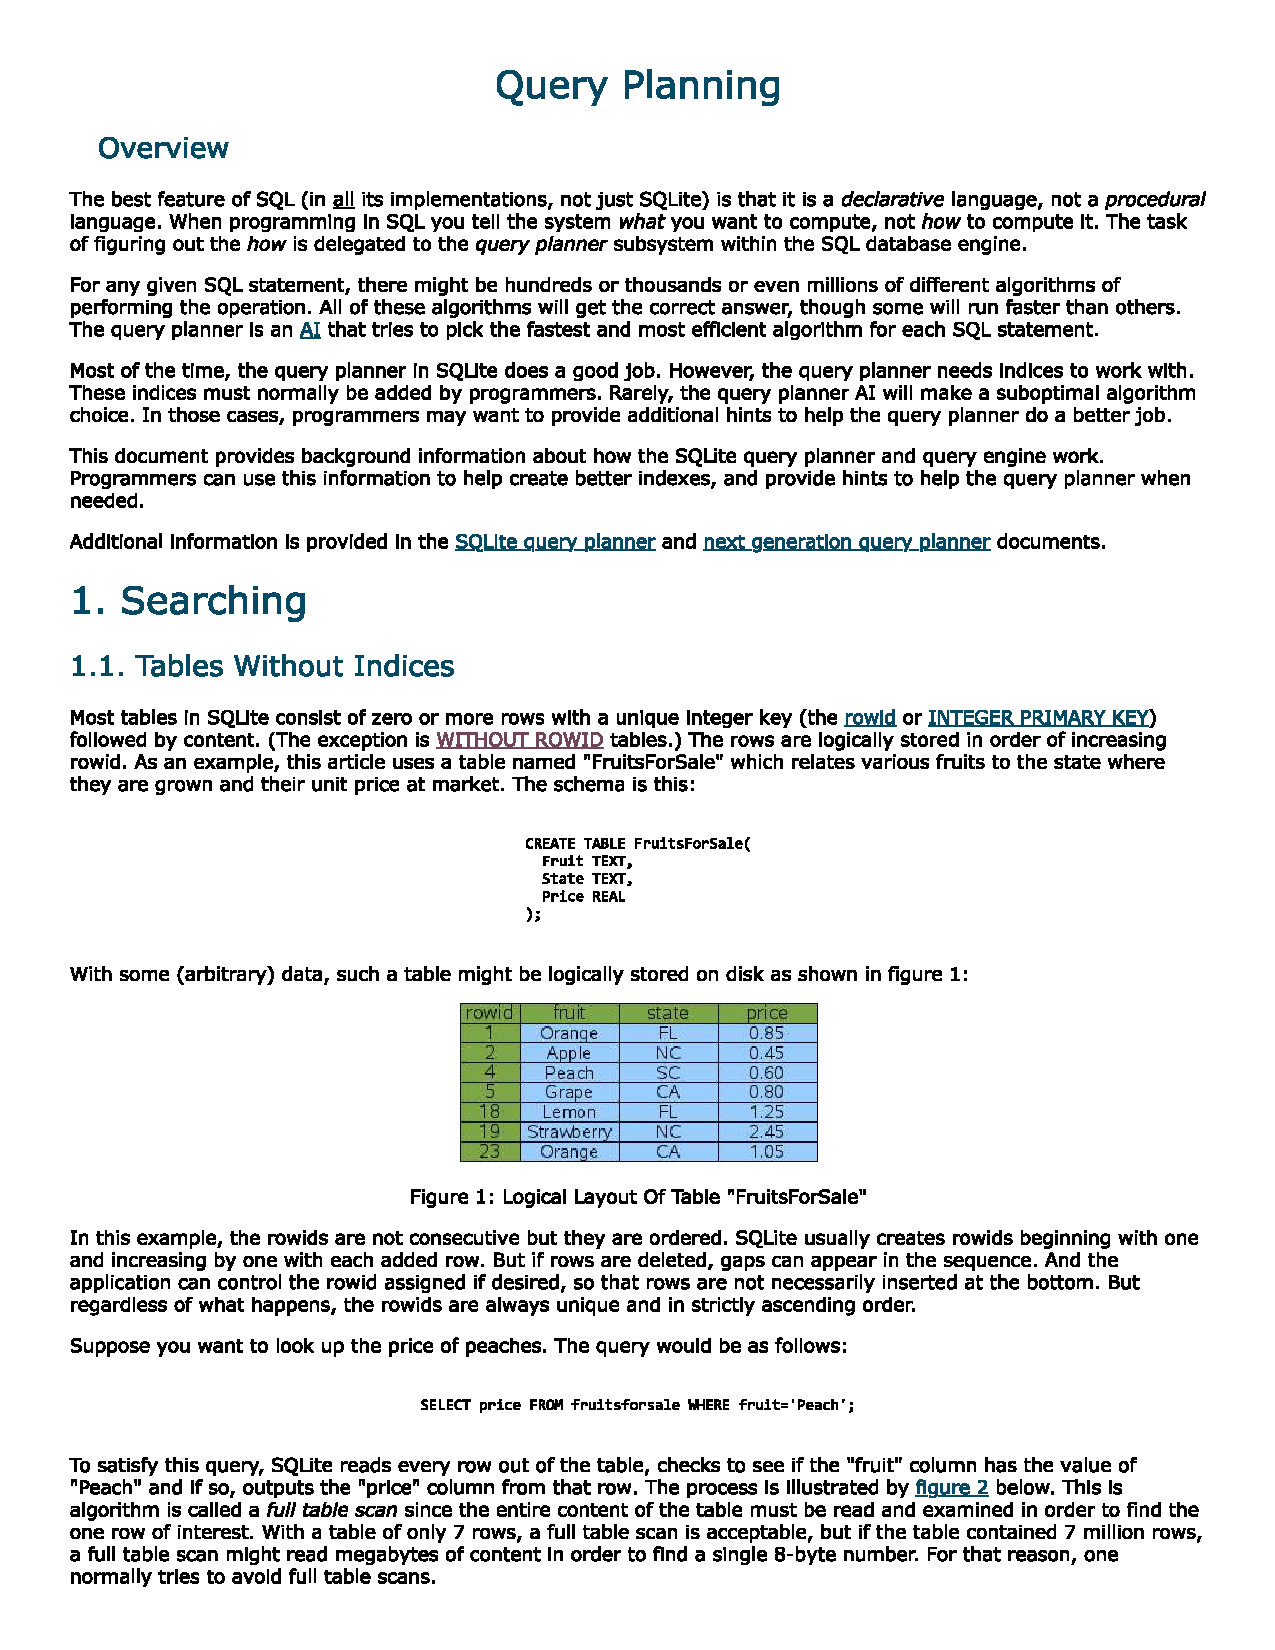
\includepdf[scale=1.0,pages={-},pagecommand={\thispagestyle{fancy}},link=true]{Query_Planning.pdf}

\end{document}